%!TEX encoding = UTF-8 Unicode
%!TEX TS-program = xelatex
\documentclass[output=paper]{langsci/langscibook}
%%\usepackage{hyperref}  already in use!

\title{Multiword expressions in an {LFG} grammar for {N}orwegian}
\author{Helge Dyvik\affiliation{University of Bergen}\and Gyri Smørdal Losnegaard\affiliation{University of Bergen}\lastand Victoria Rosén\affiliation{University of Bergen}}

%% \newcommand{\eabox}[2][-.7\baselineskip]{
%%  \ea
%%    \parbox[t]{.8\textwidth}{
%%      \vspace{#1}
%%      #2
%%     }
%%  \z
%% }

%% \newcommand{\exbox}[2][-.7\baselineskip]{
%%  \ex
%%    \parbox[t]{.8\textwidth}{
%%      \vspace{#1}
%%      #2
%%     }
%% }
\hyphenation{struc-ture hier-ar-chi-cal ADVcmt Christ-church leksikalsk-funk-sjonell Indur-khya English}
% \chapterDOI{} %will be filled in at production
%\bibliography{dyviketal} % in preamble of main file

%\epigram{“You speak an infinite deal of nothing.”
%- William Shakespeare, The Merchant of Venice}
\abstract{This chapter describes the analysis of multiword expressions in NorGram, an LFG grammar of Norwegian.
All multiword expressions need to be accounted for in the lexicon, but in different ways depending on the flexibility of the expression.
Each multiword expression is provided with a lexical entry that has a special predicate name  incorporating the lexical items that the multiword consists of and that specifies the argument structure of the predicate.
In this way, analyses are provided for a wide range of multiword types, including fixed expressions, phrasal verbs, verbal idioms, and others.
}
\maketitle
\begin{document}

\section{Introduction}\label{dyv:sec:intro}

%NOTES:
%
%In a lexicalized \isi{grammar} like \isi{LFG}, all multiword expressions need to be accounted for in the lexicon, but in different ways depending on the \isi{flexibility} of the expression.
%As a matter of principle they should be handled in the simplest way possible.
%Expressions that are really fixed may be treated in the same way as simplex words.
%Expressions that are more flexible need to allow for various inflections and need to have specifications related to \isi{subcategorization}.
%

In this chapter\footnotetext[1]{The authors have contributed equally and are listed in alphabetical order.}\addtocounter{footnote}{1} we show how multiword expressions (MWEs) are represented in NorGram, a hand-written computational \isi{grammar} of \ili{Norwegian} \citep{dyvik00en}. 
The \isi{grammar} is couched in the Lexical-Functional Grammar (\isi{LFG}) formalism \citep{bresnanlfs,dalrymplelfg}.
It was first developed in the context of the Parallel Grammar Project (ParGram), an international cooperative effort to develop parallel \isi{LFG} grammars for a number of languages \citep{pargram02}.
The Xerox Linguistic Environment (XLE) is the platform we use for \isi{grammar} development and parsing \citep{maxwell93}.

NorGram contains about 380 complex syntactic rules, corresponding to a transition network with more than 160,000 states and more than 4.7 million arcs.
The lexicon comprises approximately 180,000 lemmas for \ili{Norwegian} Bokmål and 110,000 lemmas for \ili{Norwegian} Nynorsk.
NorGram uses not only the \isi{grammar} rules and the lexicon but also templates to efficiently encode linguistic generalizations.
As noted in \citet[207]{dalrymple04}, templates in \isi{LFG} grammars “can play the same role in capturing linguistic generalizations as hierarchical type systems in theories like HPSG”.
Templates are for instance used to express generalizations about \isi{subcategorization} frames for verbs; there are more than 200 such verbal templates.  

NorGram analyzes several types of MWEs, including fixed and flexible expressions.
The classification of MWEs according to their relative \isi{flexibility} was initially proposed for \ili{English} \citep{sag02, baldwin10}, presupposing that MWEs with the same degree of \isi{flexibility} may receive the same or similar treatment in NLP systems.
The distinction between fixed, semi-fixed and syntactically flexible MWEs may thus be useful also for other languages than \ili{English}, although the criteria for distinguishing between the classes may vary.

Fixed MWEs are found in most languages with MWEs and in basically every part of speech.
These are expressions that are completely invariable, with no morphosyntactic variation or internal modification, such as the adverb \emph{by the way} and the determiner \emph{each and every}. 
Semi-fixed MWEs, as defined for \ili{English}, allow some lexical and morphological variation such as limited internal modification and inflection, while the relative word order of the components does not change.  
Examples are compound nominals (\emph{chicken soup}), proper names, such as \emph{Donald Duck}, and the subset of verbal \isi{idioms} with fixed word order, such as \emph{shoot the breeze} `chat' and \emph{kick the bucket} `die'.
Syntactically-flexible expressions display a wider range of \isi{flexibility}, allowing some or all types of syntactic variation including \isi{passivization}, \isi{relativization} and other operations that are not possible in semi-fixed MWEs.
All flexible MWEs are verbal. 
They include \isi{verb-particle constructions}, light verbs, and the subset of verbal \isi{idioms} whose word order is less restricted than semi-\isi{fixed expressions}. 
Table~\ref{dyv:tab:mweiness:flexibilityclasses} illustrates how common types of \ili{English} MWEs distribute over these classes.

\begin{table}
  \begin{tabular}{lll}
    \lsptoprule
    Flexibility class & Type & Example MWE \\
    \midrule
	Fixed &  & \emph{by the way} \\\tablevspace
	Semi-fixed & Compound nominals  & \emph{chicken soup} \\
	& Proper names & \emph{Donald Duck} \\
	& Non-decomposable \isi{idioms} & \emph{kick the bucket} \\\tablevspace
	Flexible & \isi{verb-particle constructions} &  \emph{give up} \\
	& Light verbs & \emph{give a speech} \\
	& Decomposable \isi{idioms} & \emph{spill the beans} \\
    \lspbottomrule
  \end{tabular}
  \caption{Classes of flexibility}
  \label{dyv:tab:mweiness:flexibilityclasses}
\end{table}

%The syntactic viation in \isi{verbal MWEs} in \ili{English} has fostered a theory of semantic \isi{decomposability} \cite{nunberg94} that has induced widespread attention to the relation between the syntax and semantics of \isi{verbal MWEs}.
The syntactic variation in \isi{verbal MWEs} in \ili{English} has given rise to a theory of semantic \isi{decomposability} \citep{nunberg94} which has led to increased interest in the relation between the syntax and semantics of \isi{verbal MWEs}.
Semantic decomposability is a measure of whether the meaning of the expression distributes over the MWE components or only relates to the expression as a whole.
It may explain why individual parts of an expression may be fronted, topicalized, and relativized, and may also in other ways contribute meaningfully to the information structure of the sentence.
On the other hand, semantic non-\isi{decomposability} blocks compositional interpretations, which again explains why semi-fixed MWEs are not subject to operations that would normally indicate that their components are associated with some independent meaning.

While a distinction between semantically decomposable and nondecomposable verbal \isi{idioms} may also hold for \ili{Norwegian}, the correlation between syntactic \isi{flexibility} and semantic \isi{decomposability} seems less conspicuous than for \ili{English}.
In particular, \ili{Norwegian} has subject-verb inversion in interrogative main clauses, so that the word order will vary in MWEs that are otherwise highly restricted. 
Most verbal \isi{idioms} may also undergo at least some modification (e.g., impersonal passives).
%The correlation between syntactic \isi{flexibility} and semantic \isi{decomposability} in \ili{Norwegian} verbal \isi{idioms} is thus less conspicuous than for \ili{English}.
Furthermore, the mechanisms for representing restrictions and variation in NorGram are technically the same for semi-fixed and flexible MWEs. 
Since no distinction is reflected in the way \isi{verbal MWEs} are represented in the lexicon and \isi{grammar}, all such MWEs are considered flexible, 
and MWEs with similar morphosyntactic properties are accounted for with templates which are in effect mini-grammars for subsets of MWEs.
%, for instance verb-object combinations with the same restrictions on number, definiteness and modifiability, 

With respect to subtypes of MWEs, the types of MWEs analyzed by NorGram more or less correspond to the types in Table~\ref{dyv:tab:mweiness:flexibilityclasses}, with a few exceptions. 
As in many other Germanic languages, compound nominals in \ili{Norwegian} form single graphical words. 
These are thus not considered multiword expressions.
In addition to \isi{prepositional verbs}, NorGram analyzes nouns and adjectives with selected prepositions as MWEs.
Expressions that are completely regular on the morphological and syntactic levels, such as light verb constructions, are analyzed compositionally by the \isi{grammar} and are not represented in the lexicon as MWEs.
A special case is complex numerals such as \emph{hundre og to} `one hundred two' and  \emph{to og nitti} `ninety two', which may also be considered a subtype of MWE.
The particular syntax and semantics of such expressions is accounted for with a special set of lexical entries and syntactic rules.

NorGramBank, a large parsebank for \ili{Norwegian}, has been created by parsing a corpus with NorGram \citep{dyvik16}.
Because of lexical and syntactic ambiguity, parsing with NorGram often results in many analyses for each sentence, and efficient disambiguation is therefore necessary.
The INESS project\footnote{\url{http://clarino.uib.no/iness}} has developed a treebanking infrastructure for parsing, disambiguating, storing, and searching the texts in NorGramBank \citep{rosen12lrec}.
The parsebank currently consists of about 60 million words of analyzed text, of which sentences covering 350,000 words have been manually disambiguated by computer-generated discriminants \citep{rosen07lfg}.
The remainder of the corpus has been stochastically disambiguated.
INESS Search is a tool for searching in \isi{LFG} and other \isi{treebanks} in the treebanking infrastructure \citep{meurer12}.
MWEs are analyzed by NorGram in such a way that the different types may be searched for.

The original lexical resource used for the NorGram lexicon, NorKompLeks, contained a small number of \isi{fixed expressions} \citep{nordgard00}.
The main design of the treatment of MWEs in NorGram was developed during ParGram \citep{pargram02} and especially during the LOGON machine translation project \citep{lonning04}.
A large number of MWEs have been added to NorGram’s lexicon during the construction of NorGramBank.
When annotators discovered MWEs that did not receive an analysis or that received an incorrect analysis, they constructed new lexical entries or edited existing lexical entries as needed in order to cover the MWEs \citep{losnegaard12,rosen16lre}.

This chapter is organized as follows.
In Section~\ref{dyv:sec:mweiness:LFG} an overview of the basics of \isi{LFG} is given, showing how constructions without MWEs are analyzed in NorGram as a background for the treatment of MWEs in the following sections.
Section~\ref{dyv:sec:mweiness:fixed} illustrates the analysis of \isi{fixed expressions}, while Section~\ref{dyv:sec:mweiness:flexexp} is about the analysis of flexible expressions, including \isi{phrasal verbs}, verbal \isi{idioms}, and nonverbal flexible expressions.
Section~\ref{dyv:sec:mweiness:variation} shows how various syntactic modifications are handled, including intervening words, \isi{long-distance dependencies} and passive alternations.
Section~\ref{dyv:sec:mweiness:complementation} discusses numerous complex complementation patterns that are covered by NorGram for \ili{Norwegian} MWEs.
Section~\ref{dyv:sec:mweiness:conc} presents our conclusions.

\section{Syntactic analysis in LFG}\label{dyv:sec:mweiness:LFG}

\isi{LFG} analyses have two distinct levels of syntactic representation: constituent structure (c-structure) and functional structure (f-structure).
The c-structure is a \isi{phrase} structure tree that represents precedence and dominance relations.
The f-structure is an attribute-value matrix with information about grammatical functions such as subject and object and grammatical features such as tense, gender and number.
An example of a NorGram analysis of the sentence in (\ref{dyv:ex:mweiness:thinking-while-on-bus}) is given in Figure~\ref{dyv:fig:mweiness:thinking-while-on-bus}.\footnote{In this example the morphological structure of the word form \textit{bussen} is indicated since it is relevant for the analysis being discussed.
Otherwise, we simplify the glossing by omitting morpheme-by-morpheme analysis and using two \ili{English} words to render one \ili{Norwegian} word when necessary.}
%In this and subsequent examples the words making up the MWE are highlighted with boldface.
%\ea\label{dyv:ex:mweiness:thinking-while-on-bus}
%\gll Hun \textbf{tenkte} \textbf{på} bussen. \\
%     she thought on {the bus}\\
%\glt `She was thinking (while) on the bus./She thought about the bus.’
%\z

\ea\label{dyv:ex:mweiness:thinking-while-on-bus}
\gll Hun tenkte på buss-en. \\
     she thought on bus-{\definite}.{\sg}\\
\glt `She was thinking (while) on the bus./She thought about the bus.’
\z

\begin{figure}
  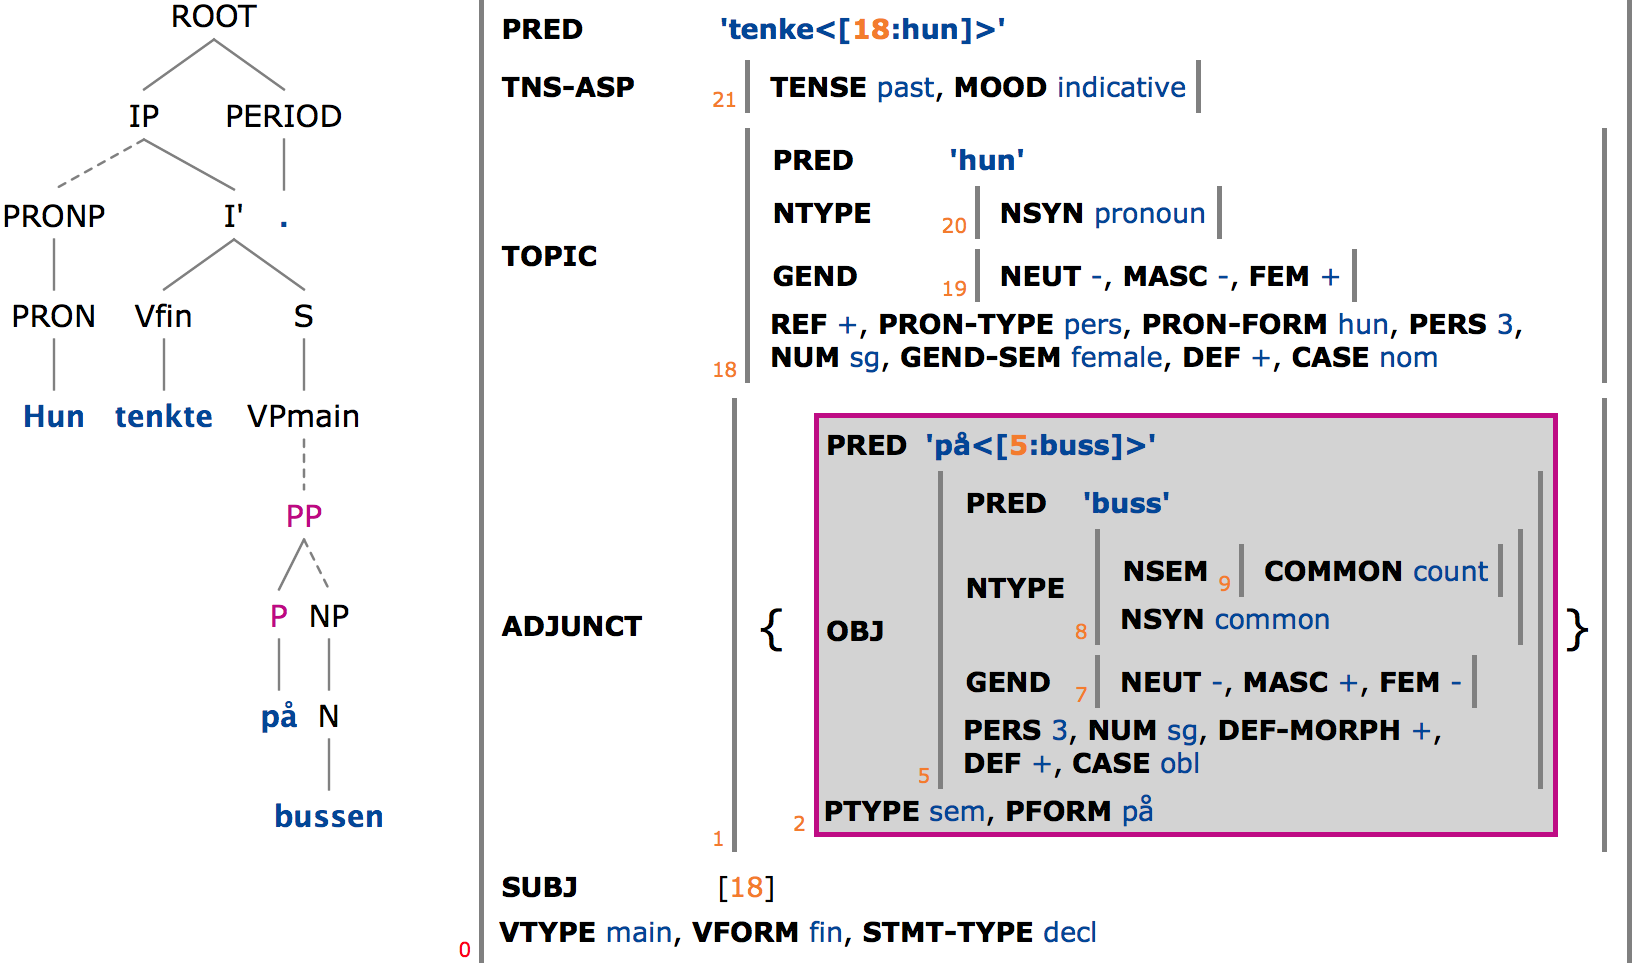
\includegraphics[width=\textwidth]{figures/tenke-paa-bussen-highlight.png}
  \caption{C- and f-structure for \textit{Hun tenkte på bussen}.}
  \label{dyv:fig:mweiness:thinking-while-on-bus}
\end{figure}

This sentence is ambiguous, as shown by the two idiomatic translations.
The analysis in Figure~\ref{dyv:fig:mweiness:thinking-while-on-bus} concerns the first translation, where the prepositional \isi{phrase} \textit{på bussen} `on the bus' is an \isi{adjunct} (adverbial).
The second reading, where \textit{tenke på} `think about’ is a phrasal verb, will be treated in Section~\ref{dyv:sec:mweiness:flexexp}.

The \isi{phrase} structure rules and lexicon of an \isi{LFG} \isi{grammar} assign the c-struc\-ture.
NorGram uses a version of X’-syntax that is inspired by \citet{bresnanlfs}, with some adjustments which depart from strictly binary branching structures.

The f-structure is projected from the c-structure by the functional description (f-description), which describes correspondences between the two levels.
%Functional annotations in the \isi{phrase} structure rules and the lexical entries describe parts of the f-structure.
One such correspondence is illustrated in Figure~\ref{dyv:fig:mweiness:thinking-while-on-bus} by the highlighting of the PP node and the corresponding partial f-structure.
The \isi{phrase} structure rules that assign this f-structure are given in (\ref{dyv:ex:mweiness:PP-rule}) and (\ref{dyv:ex:mweiness:NP-rule}).
The rule daughters are listed vertically after the horizontal arrow, with each node's functional annotations following after a colon.\footnote{The examples of rules, lexical entries, and templates in the following are simplified for the purpose of exposition. Neither the format nor the content is exactly the same as in NorGram.}

\ea\label{dyv:ex:mweiness:PP-rule}
{\small 
PP	$\rightarrow$	P: $\uparrow$=$\downarrow$ \\
\hspace{2.3em} NP: ($\uparrow$~OBJ)=$\downarrow$
}
\z

\ea\label{dyv:ex:mweiness:NP-rule}
{\small 
NP	$\rightarrow$	N: $\uparrow$=$\downarrow$ \\
}
\z

The annotations on the rule daughters describe the associated f-structures.
In the equations, $\uparrow$ refers to the f-structure of the mother node (the category on the left-hand side of the rule), while $\downarrow$ refers to the f-structure of the daughter node (the category carrying the annotation on the right-hand side of the rule).
Thus the equation $\uparrow$=$\downarrow$ annotated to a rule daughter means that the daughter node and its mother node will project the same f-structure.
The equation ($\uparrow$~OBJ)=$\downarrow$ on the NP node in (\ref{dyv:ex:mweiness:PP-rule}) specifies that the f-structure of the mother node (PP) has an object (OBJ) which is the f-structure of the daughter node (NP).
In this way the highlighted f-structure with the index ``2'' at its lower left corner in Figure~\ref{dyv:fig:mweiness:thinking-while-on-bus} is projected from the PP node.
Both the PP node and the P node are highlighted in the c-structure since they both project this same f-structure.

The annotations on the \isi{phrase} structure rules account for only part of the information in the f-structure.
Other information comes from the word forms in the terminal nodes of the tree.
For instance, the lexical and morphological information for the word \textit{bussen} contributes all the equations in (\ref{dyv:ex:mweiness:f-descr-bussen}).
These equations are part of the f-description for the f-structure that is the value of the OBJ attribute (with the index ``5'') in Figure~\ref{dyv:fig:mweiness:thinking-while-on-bus}.

%The annotations on the \isi{phrase} structure rules account for only part of the information in the f-structure.
%Other information comes from the word forms in the terminal nodes of the tree.
%The equations in (\ref{dyv:ex:mweiness:f-descr-bussen}) constitute the f-description of the f-structure that is the value of the OBJ attribute (with the index `5') in Figure~\ref{dyv:fig:mweiness:thinking-while-on-bus}.
%All these equations except for ($\uparrow$~CASE)=obl are contributed by the word \textit{bussen}.

%A simple \isi{lexical entry} for \textit{bussen} could be as in (\ref{dyv:ex:mweiness:lexentry-bussen}).
%Lexical entries for \textit{på} and \textit{buss} are provided in (\ref{dyv:ex:mweiness:lexentry-paa}) and (\ref{dyv:ex:mweiness:lexentry-buss}).
%The \isi{lexical entry} for \textit{buss} is provided in (\ref{dyv:ex:mweiness:lexentry-buss}).

%\ea\label{dyv:ex:mweiness:lexentry-buss}
%buss \hspace{0.5em} N \hspace{0.5em} XLE \hspace{0.5em} @(COUNTNOUN buss).
%\z

\ea\label{dyv:ex:mweiness:f-descr-bussen}
{\small 
($\uparrow$~PRED)=`buss' \\
($\uparrow$~NTYPE NSEM COMMON)=count \\
($\uparrow$~NTYPE NSYN)=common \\
($\uparrow$~GEND NEUT)=$-$ \\
($\uparrow$~GEND MASC)=$+$ \\
($\uparrow$~GEND FEM)=$-$ \\
($\uparrow$~PERS)=3 \\
($\uparrow$~NUM)=sg \\
($\uparrow$~DEF-MORPH)=$+$ \\
($\uparrow$~DEF)=$+$ \\
%($\uparrow$~CASE)=obl \\
}
\z

%All except for the first one are common to many other nouns.
The first equation, which assigns the PRED(icate) value `buss', is specific to this noun, but the others are common to many other words.
Some of the equations come from features assigned to the word form \textit{bussen} by the morphological analyzer run prior to parsing; these features are +Noun, +Sg, +Def and +Masc, and they will appear in the string presented to the syntactic parser.
Other equations come from the \isi{lexical entry} for the noun  \textit{buss}.
Both the features and the noun must have entries in the lexicon;  these are shown in (\ref{dyv:ex:mweiness:entry-noun})--(\ref{dyv:ex:mweiness:entry-buss}).
Each \isi{lexical entry} specifies a lexical category; SUFF (for suffix) is the category for morphological features.
%Both the features and the noun must have entries in the NorGram lexicon;  (\ref{dyv:ex:mweiness:entry-noun})--(\ref{dyv:ex:mweiness:entry-masc}) shows possible lexical entries for the features, while (\ref{dyv:ex:mweiness:entry-buss}) provides an entry for the noun.

\ea\label{dyv:ex:mweiness:entry-noun}
{\small 
$+$Noun \hspace{0.4em} SUFF \hspace{0.4em} ($\uparrow$~PERS)=3
}
\z

\ea\label{dyv:ex:mweiness:entry-sg}
{\small 
$+$Sg \hspace{1.7em} SUFF \hspace{0.4em} ($\uparrow$~NUM)=sg
}
\z

\ea\label{dyv:ex:mweiness:entry-def}
{\small 
$+$Def  \hspace{1.2em} SUFF \hspace{0.4em} @DEF
}
\z
%\ea\label{dyv:ex:mweiness:entry-def}
%$+$Def \hspace{1.2em} ($\uparrow$~DEF-MORPH)=$+$ \\
%\hspace{3.5em}  ($\uparrow$~DEF)=$+$ \\
%\z

\ea\label{dyv:ex:mweiness:entry-masc}
{\small 
$+$Masc  \hspace{0.6em} SUFF \hspace{0.4em} @MASC
}
\z

%\ea\label{dyv:ex:mweiness:entry-masc}
%$+$Masc \hspace{0.6em} ($\uparrow$ GEND MASC)=$+$ \\
%\hspace{3.5em}  ($\uparrow$ GEND FEM)=$-$ \\
%\hspace{3.5em}  ($\uparrow$ GEND NEUT)=$-$ \\
%\z

\ea\label{dyv:ex:mweiness:entry-buss}
{\small 
buss  \hspace{1.5em} N \hspace{1.8em} @(COUNTNOUN buss)
}
\z

%\ea\label{dyv:ex:mweiness:entry-buss}
%buss \hspace{1.4em} ($\uparrow$ PRED)=`buss' \\
%\hspace{3.5em}  ($\uparrow$ NTYPE NSEM COMMON)=count \\
%\hspace{3.5em}  ($\uparrow$ NTYPE NSYN)=common \\
%\z

The equations in the first two entries each contribute one attribute-value pair to the f-structure.
Entries (\ref{dyv:ex:mweiness:entry-def})--(\ref{dyv:ex:mweiness:entry-buss}) contain \isi{template} invocations rather than equations.
The @-sign indicates a call to a \isi{template}, while DEF, MASC and COUNTNOUN are names of templates.
A \isi{template} is an f-description, a collection of equations which it is convenient to refer to by a name rather than listing all the equations.
Templates can be used in different places in the \isi{grammar} and lexicon, and \isi{template} definitions may refer to other templates.

The definition of the \isi{template} named DEF is shown in (\ref{dyv:ex:mweiness:def-template}).
All nouns inflected in the definite form will carry these two equations, so it can be convenient to refer to them together.
%They can be factored out into a \isi{template}, a named f-description, as in (\ref{dyv:ex:mweiness:def-template}).

\ea\label{dyv:ex:mweiness:def-template}
{\small 
DEF = \\
\hspace{2em}  ($\uparrow$~DEF-MORPH)=$+$ \\
\hspace{2em}  ($\uparrow$~DEF)=$+$ \\
}
\z

%The \isi{lexical entry} for the morphological feature \textit{$+$Def} can therefore be specified as in (\ref{dyv:ex:mweiness:def-entry}).

%\ea\label{dyv:ex:mweiness:def-entry}
%$+$Def  \hspace{1.2em} @DEF
%\z

\ili{Norwegian} has a complicated system of gender agreement because of some nouns that may have either masculine or feminine agreement, and because adjectives and determiners may be unspecified for certain gender distinctions.
To account for this, each noun must receive a plus or minus value for each of the three genders.
The equations needed for specifying masculine gender are included in the \isi{template} in (\ref{dyv:ex:mweiness:masc-template}).
These equations do not simply describe attribute-value pairs; they describe paths through the f-structure.
The equation ($\uparrow$ GEND MASC)=$+$ states that the f-structure has an attribute GEND which has as its value a subsidiary f-structure which in its turn has an attribute MASC with the value $+$.

\ea\label{dyv:ex:mweiness:masc-template}
{\small 
MASC = \\
\hspace{2em}  ($\uparrow$ GEND MASC)=$+$ \\
\hspace{2em}  ($\uparrow$ GEND FEM)=$-$ \\
\hspace{2em}  ($\uparrow$ GEND NEUT)=$-$ \\
}
\z

%\ea\label{dyv:ex:mweiness:masc-template}
%\verb§MASC =§\\
%\verb§    (§$\uparrow$\verb§ GEND MASC)=§$+$\\
%\verb§    (§$\uparrow$\verb§ GEND FEM)=§–\\
%\verb§    (§$\uparrow$\verb§ GEND NEUT)=§$-$
%\z
%
%\setlength{\tabcolsep}{0.1em} % for the horizontal padding
%\ea\label{dyv:ex:rules}
%\begin{tabular}{ll}
%I' $\rightarrow$ &  Vfin: $\uparrow$=$\downarrow$\\
% & (S: $\uparrow$=$\downarrow$).\\\\
%\end{tabular}
%\z
%
%\setlength{\tabcolsep}{0.1em} % for the horizontal padding
%\eabox{\label{dyv:ex:rules}
%\begin{tabular}{ll}
%I' $\rightarrow$ &  Vfin: $\uparrow$=$\downarrow$\\
% & (S: $\uparrow$=$\downarrow$).\\\\
%\end{tabular}}
%
%\ea\label{dyv:ex:rules}
%\begin{tabular}{lll}
%I' $\rightarrow$ &  Vfin: & $\uparrow$=$\downarrow$\\
% & (S: & $\uparrow$=$\downarrow$).\\\\
%\end{tabular}
%
%\begin{tabular}{lll}
%S $\rightarrow$ &  (PRONP: & ($\uparrow$ SUBJ)=$\downarrow$\\
%& &@SUBJCASE\\
%& [...]\\
%& (PRONrfl: & \{ \enspace ($\uparrow$ OBJ-BEN)=$\downarrow$\\
%& & | \enspace ($\uparrow$ OBJ)=$\downarrow$ \enspace \} \\
%& [...]\\
% & (ADVPs+: & $\downarrow$ ∈ ($\uparrow$ ADJUNCT))\\
%& [...]\\
%& (APsmpl:  & $\downarrow$ ∈ ($\uparrow$ ADJUNCT))\\
%& [...]\\
% & (VPmain: & $\uparrow$=$\downarrow$)\\
%& [...].\\\\
%\end{tabular}
%
%\begin{tabular}{lll}
%VPmain $\rightarrow$ & [...]\\
%& (PRTP: & $\uparrow$=$\downarrow$\\
%& & ($\uparrow$ CHECK PRT-VERB)=c +)\\
%& [...].\\\\
%\end{tabular}
%\z
%


Like the \isi{template} MASC, the \isi{template} COUNTNOUN also describes paths through the f-structure.
The NTYPE SYN features distinguish between common nouns, proper nouns, pronouns, etc. while the NTYPE SEM COMMON features distinguish between count nouns, mass nouns, etc.
All nouns must contribute a PRED feature to the f-structure, but the PRED feature itself will differ from noun to noun.
The \isi{template} in (\ref{dyv:ex:mweiness:countnoun-template}) is parameterized; the parameter P will be substituted by the argument supplied in the invocation of the \isi{template}, for example the word \textit{buss} in (\ref{dyv:ex:mweiness:entry-buss}).
%All count nouns have in common certain NTYPE features.
%All count nouns must also contribute a PRED feature to the f-structure, but the PRED feature itself will differ from noun to noun.
%The \isi{template} in (\ref{dyv:ex:mweiness:countnoun-template}) is parameterized; the parameter P will be substituted by the argument supplied in the invocation of the \isi{template}.
%For the \isi{lexical entry} in (\ref{dyv:ex:mweiness:entry-buss}), the argument \textit{buss} will be substituted for P, providing the PRED value `buss'.


\ea\label{dyv:ex:mweiness:countnoun-template}
{\small 
COUNTNOUN (P) = \\
\hspace{2em}  ($\uparrow$ PRED)=P \\
\hspace{2em}  ($\uparrow$ NTYPE NSEM COMMON)=count \\
\hspace{2em}  ($\uparrow$ NTYPE NSYN)=common \\
}
\z

The value of a PRED attribute is a semantic form.
A semantic form is always enclosed in single quotation marks, indicating that the value is unique, which means that it cannot be unified even with an identical-looking value of some other attribute.
For some words the semantic form includes not only the word itself, but also a syntactic argument list.
This is the case for two of the words in \textit{hun tenker på bussen} (in the interpretation being considered in this section).
The verb has the semantic form `tenke<[SUBJ]>', meaning that the verb is intransitive and subcategorizes only for a subject, and the preposition has the semantic form `på<[OBJ]>', indicating that it requires an object.
%This is the case for two of the words in (\ref{dyv:ex:mweiness:thinking-while-on-bus}); the verb has the semantic form `tenke<[SUBJ]>', meaning that the verb subcategorizes for a subject, and the preposition has the semantic form `på<[OBJ]>', indicating that it requires an object.

Verbs can of course subcategorize for several arguments.
For example, the verb \textit{slå} `hit' has the semantic form `slå<[SUBJ,OBJ]>' since it requires a subject and an object.
The completeness requirement for f-structures stipulates that each of the syntactic functions mentioned in the semantic form of a PRED feature must occur on the same level of f-structure as that PRED.
There is also a coherence requirement to the effect that subcategorizable syntactic functions may only occur on the same level of f-structure as a PRED feature if they are mentioned in its semantic form.
The argument lists in semantic forms are thus crucial for determining grammaticality.
The semantic forms ``govern the process of semantic interpretation” \citep[177]{kaplanbresnan82}.

The crucial challenge of representing MWEs is that they defy normal compositional analysis.
The \isi{LFG} solution that is implemented in NorGram is to assign to each MWE a special \isi{lexical entry} that has its own PRED value and thus its own argument structure.
Each MWE has a semantic form with a special predicate name and a list of any syntactic arguments that this predicate requires.
%This approach makes it possible to have a clear separation between the 
This will be shown in detail for the various types of MWEs in the following sections.
%This \isi{template} can be invoked in the \isi{lexical entry} in (\ref{dyv:ex:mweiness:def-entry}).

%\ea\label{dyv:ex:mweiness:entry-def-new}
%$+$Def  \hspace{1.2em} @DEF
%\z
%
%\ea\label{dyv:ex:mweiness:entry-masc-new}
%$+$Masc  \hspace{1.2em} @MASC
%\z
%
%\ea\label{dyv:ex:mweiness:entry-buss-new}
%buss  \hspace{1.2em} @(COUNTNOUN buss)
%\z


%\ea\label{dyv:ex:mweiness:f-descr-bussen}
%bussen \hspace{0.5em} ($\uparrow$~PRED)=`buss' \\
%\hspace{3.6em}  ($\uparrow$~NTYPE NSEM COMMON)=count \\
%\hspace{3.6em}  ($\uparrow$~NTYPE NSYN)=common \\
%\hspace{3.6em}  ($\uparrow$~GEND NEUT)=- \\
%\hspace{3.6em}  ($\uparrow$~GEND MASC)=+ \\
%\hspace{3.6em}  ($\uparrow$~GEND FEM)=- \\
%\hspace{3.6em}  ($\uparrow$~PERS)=3 \\
%\hspace{3.6em}  ($\uparrow$~NUM)=sg \\
%\hspace{3.6em}  ($\uparrow$~DEF-MORPH)=+ \\
%\hspace{3.6em}  ($\uparrow$~DEF)=+ \\
%\z

%This entry includes all the information passed to the f-structure by the word form \textit{bussen}.
%But since NorGram is used with a morphological analyzer, the lexicon does not need to have full-form entries. The equations for gender, person, number and definiteness are all provided through the morphological analysis.
%This means that the entry 
%Although the usual display in XLE-Web does not show sublexical features, clicking on a preterminal node expands the view to display those features.
%We see this view of the word \textit{bussen} in (\ref{dyv:fig:mweiness:sublexical}).
%The morphological features \textit{+Noun}, \textit{+Masc}, \textit{+Sg} and \textit{+Def} have entries in the lexicon, as shown in ().
%
%\begin{figure}
%  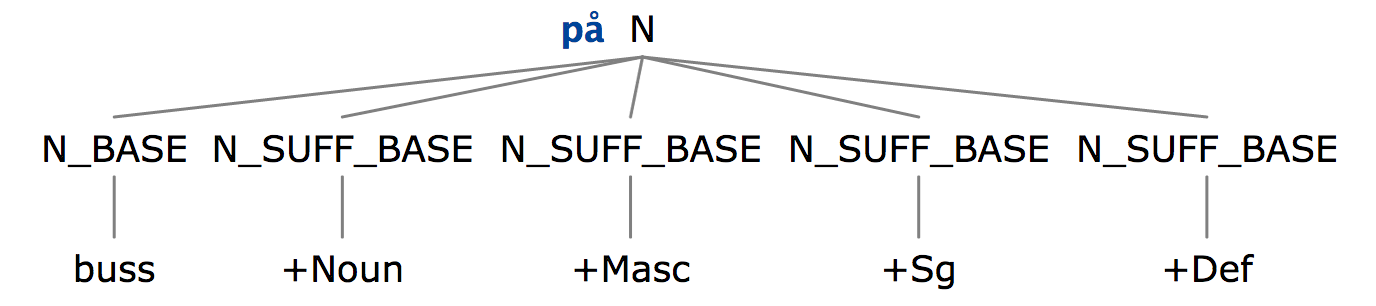
\includegraphics[width=0.7\textwidth]{figures/sublexical.png}
%  \caption{Sublexical features for \textit{bussen}.}
%  \label{dyv:fig:mweiness:sublexical}
%\end{figure}
%
%\ea\label{dyv:ex:mweiness:sublexicalentries}
%+Noun \hspace{0.5em} ($\uparrow$~PERS)=3 \\
%+Masc \hspace{0.7em} @MASC \\
%+Sg \hspace{1.8em} ($\uparrow$~NUM)=sg \\
%+Def \hspace{1.3em} @DEF \\
%\z
%
%The entries for \textit{+Noun} and \textit{+Sg} each contribute one equation.
 
 \section{Fixed expressions}\label{dyv:sec:mweiness:fixed}

Fixed expressions, such as \textit{ad hoc}, \textit{déjà vu}, and \textit{vice versa}, are those that do not vary with respect to inflection and that do not admit any internal modification.
They are also called inflexible expressions or ``words with spaces''.
Fixed expressions are the simplest MWEs to implement; they are entered into the NorGram lexicon as single graphical words containing white space, so they are literally treated as words with spaces.

\ea\label{dyv:ex:mweiness:wws}
\gll Hun likte \textbf{i} \textbf{bunn} \textbf{og} \textbf{grunn} ikke \textbf{New} \textbf{York} \textbf{i} \textbf{det} \textbf{hele} \textbf{tatt}. \\
     she liked in bottom and ground not New York in the whole taken\\
\glt `She basically didn’t like New York at all.’
\z

The sentence in (\ref{dyv:ex:mweiness:wws}) contains three such expressions: \textit{i bunn og grunn}, \textit{New York}, and \textit{i det hele tatt}.\footnote{In this and subsequent examples the lexically fixed words making up the MWE are highlighted with boldface.}
The c-structure of (\ref{dyv:ex:mweiness:wws}) is shown in Figure~\ref{dyv:fig:mweiness:wws-cstr}.
The simplified f-structure is shown in Figure~\ref{dyv:fig:mweiness:wws-fstr}; this is the ``PREDs only'' view of f-structure where feature paths that do not end in PRED values are suppressed. 
The three expressions belong to different parts of speech: ADVcmt (commitment adverb), PROP (proper noun), and ADVs (sentence adverb).
The adverbs have the function ADJUNCT in the f-structure while the proper noun functions as the OBJ.
There are numerous \isi{fixed expressions} in most parts of speech in \ili{Norwegian}.

%\ea\label{dyv:ex:mweiness:wws}
%\gll Hun likte \textbf{i} \textbf{bunn} \textbf{og} \textbf{grunn} ikke \textbf{New} \textbf{York} \textbf{i} \textbf{det} \textbf{hele} \textbf{tatt}. \\
%     she liked in bottom and ground not New York in the whole taken\\
%\glt `She basically didn’t like New York at all.’
%\z
%
\begin{figure}
  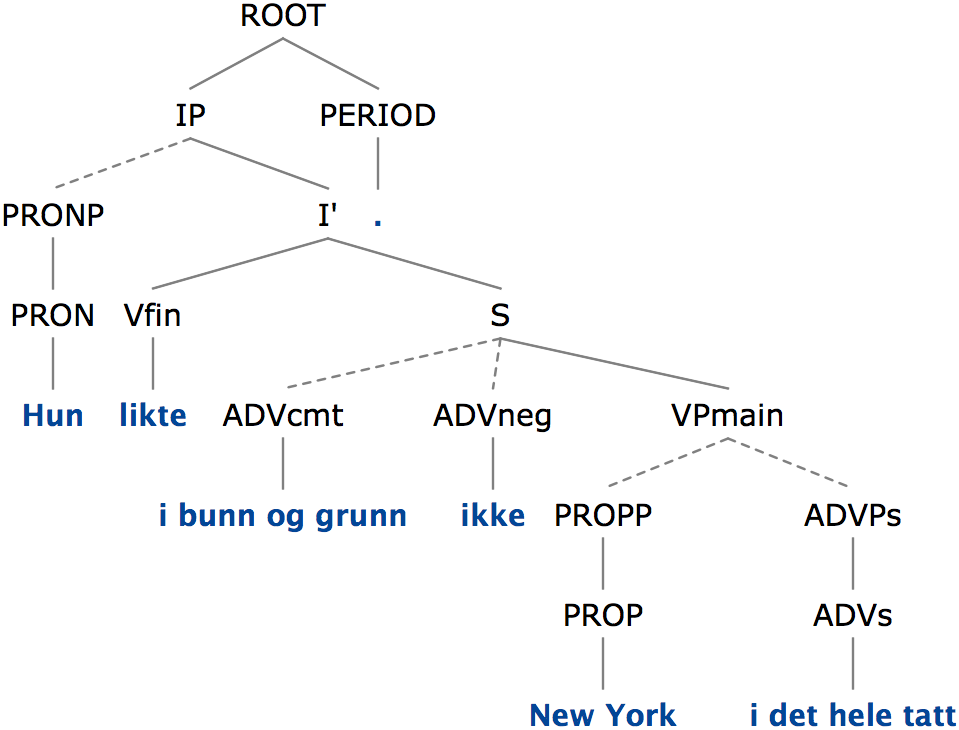
\includegraphics[width=0.6\textwidth]{figures/wws-cstr}
  \caption{C-structure for example (\ref{dyv:ex:mweiness:wws})}
  \label{dyv:fig:mweiness:wws-cstr}
\end{figure}

\begin{figure}
  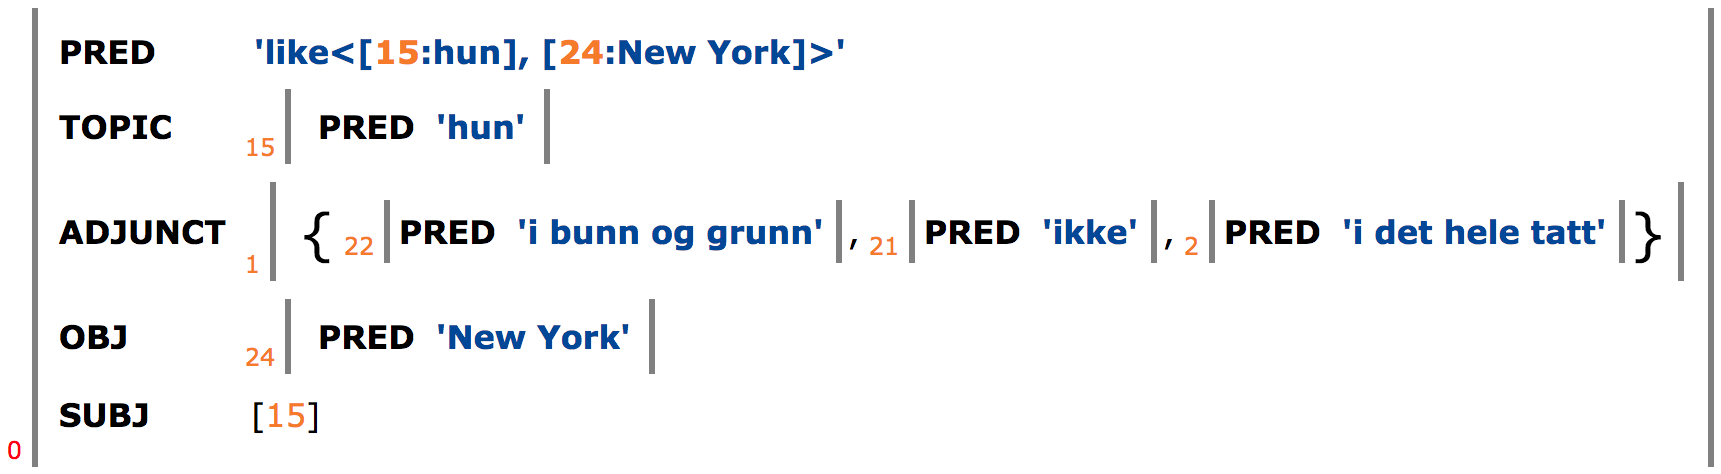
\includegraphics[width=0.9\textwidth]{figures/wws-fstr}
  \caption{F-structure for example (\ref{dyv:ex:mweiness:wws})}
  \label{dyv:fig:mweiness:wws-fstr}
\end{figure}

%Fixed expressions are easily searchable in NorGramBank.
%In the c-structure they may be found by searching for word forms that include one or more white spaces.
%The search expression \textit{``.* .*''} means: search for a word form (anything included within double quotations marks) consisting of any character (the period) zero or more times (the Kleene star) followed by a white space followed by any character zero or more times.

%NOTES:
%
%This usually includes lots about nominal compounds, which are very common in \ili{English}.
%We should perhaps point out that these are normally written as single words in \ili{Norwegian}.
%
%We do have a huge number of names that are \isi{fixed expressions}.
%Perhaps we should look into to what degree they are really fixed, see e.g. Sag et al.'s stuff about the San Francisco 49'ers, the 49'ers, etc.
%
%Prepositional MWEs
%
%determinerless-prepositional phrases (do we have any of these?) 
%
%complex prepositions (sammen med)
%
%conjunctionless coordinated PPs
%
%We also have adverbial (ansikt til ansikt), pronominal (noe som helst).
%Other types?


\section{Flexible expressions}\label{dyv:sec:mweiness:flexexp}

Flexible expressions may exhibit a great deal of syntactic variation, but in some respects they are inherently fixed or restricted.
One of the characterizing features of MWEs is that they are lexically fixed, meaning that they consist of at least two words that cannot be substituted with near-synonyms or semantically related words without the expression losing its idiomatic meaning.
The verbal idiom \emph{komme på kant med} in (\ref{dyv:ex:mweiness:kommepåkantmed}) has four such fixed lexical words.

%Flexible expressions may exhibit a great deal of syntactic variation, but in some respects they are inherently fixed or restricted.
%As one of their characterizing features, MWEs are lexically fixed with at least two fixed components that cannot be substituted with near-synonyms or semantically related words. 
%%One characterizing feature of MWEs is that they are lexically fixed, with at least two fixed components. 
%The verbal idiom \emph{komme på kant med} in (\ref{dyv:ex:mweiness:kommepåkantmed}) has four fixed lexemes.

%Treebank: nob-fn version: 2016-05-17; Document: Sandnes, Heidi Elisabeth: I skyggen av Grieg; \isi{grammar}: \ili{Norwegian} Bokmål
%Sentence #30 Hun var ikke villig til å komme på kant med det gode selskap.
\ea\label{dyv:ex:mweiness:kommepåkantmed}
\gll Hun var ikke villig til å \textbf{komme} \textbf{på} \textbf{kant} \textbf{med} det gode selskap. \\
     she was not willing to to come on edge with the good company \\
\glt `She was not willing to fall out with the in-crowd.’
\z

Flexible MWEs are often also morphosyntactically restricted, with constraints on grammatical features, on the modification of component words, and on specifiers such as quantifiers and determiners.
For instance, the noun \emph{kant} in (\ref{dyv:ex:mweiness:kommepåkantmed}) can only be in the singular indefinite form, and it does not admit any specifiers or modifiers.
%While \emph{kant} does not admit specifiers or modifiers in this expression, the PP \emph{på kant med} does. 
The PP \emph{på kant med}, however, does admit modifiers; in (\ref{dyv:ex:mweiness:modification}) the modifier \emph{helt} `completely' has scope over the entire expression.
In NorGram, no distinction is currently made in the representation of internal and (semantically) external modification of MWEs. 

\ea\label{dyv:ex:mweiness:modification}
\gll Hun \textbf{kom} helt \textbf{på} \textbf{kant} \textbf{med} det gode selskap. \\
she came fully on edge with the good society \\
\glt `She completely fell out with the in-crowd.' \\
\z
%\ea\label{dyv:ex:mweiness:modification}
%hun \textbf{kom} helt \textbf{på} \textbf{kant} \textbf{med} naboene \\
%she came fully on edge with {the neighbours} \\
%`she fell out with her neighbours completely' \\
%\z

The mechanisms for representing lexical and morphological restrictions in flexible MWEs are the same as the ones used for regular constructions.
As described in Section~\ref{dyv:sec:mweiness:LFG}, simplex words are assigned predicate values through equations in the \isi{lexical entry}, as in the entry for the simplex lexeme \emph{buss} in example (\ref{dyv:ex:mweiness:f-descr-bussen}), which has the predicate assignment equation ($\uparrow$~PRED)=`buss'. 
For words that subcategorize for other elements, such as verbs, this is done through the assignment of a \isi{predicate-argument structure} (or \isi{subcategorization} frame). 
For instance, the intransitive verb \emph{klage} `complain' is assigned a frame through the \isi{template} call @(V-SUBJ klage) in the \isi{lexical entry}, invoking the \isi{template} V-SUBJ. 
Part of this \isi{template} is shown in (\ref{dyv:ex:mweiness:verb-template}).

\ea\label{dyv:ex:mweiness:verb-template}
{\small 
 V-SUBJ (P) = \\
\hspace{2em} ($\uparrow$ PRED)=`P<($\uparrow$ SUBJ)>' \\
}
\z

The predicate value of the verb is parameterized and listed together with its arguments in the \isi{subcategorization} frame, which includes everything between quotation marks in (\ref{dyv:ex:mweiness:verb-template}).
When the \isi{template} is invoked, the lemma form \emph{klage} in the \isi{template} call replaces the parameter P. 
The equation on the second line assigns one argument, the subject, to P, yielding the predicate-argument  structure `klage<($\uparrow$~SUBJ)>' as the PRED value for the intransitive reading of this verb.


Lexical fixedness in flexible MWEs is handled through lexical selection in the entry of the subcategorizing word. 
In addition to its usual intransitive reading, the verb \emph{klage} `complain' is the syntactic head of the VP idiom \emph{klage sin nød} `pour out one's troubles', where it subcategorizes for the object noun \emph{nød} `need'. 

%Treebank: nob-novel_5 version: 2016-05-17; Document: Henriksen, Vera: Helgenkongen; \isi{grammar}: \ili{Norwegian} Bokmål
%Sentence #3447: Og hun klaget sin nød til alle som ville høre.
 \ea\label{dyv:ex:mweiness:klagesinnød}
\gll Og hun \textbf{klaget} \textbf{sin} \textbf{nød} til alle som ville høre. \\
     and she complained her need to all who wanted hear \\
\glt `And she poured out her troubles to everyone who wanted to listen.’
\z
% \ea\label{dyv:ex:mweiness:klagesinnød}
%\gll Hun \textbf{klaget} \textbf{sin} \textbf{nød} til naboene. \\
%     she complained  her need to {the neighbours} \\
%\glt `She complained to the neighbours.’
%\z

Lexical entries for VP \isi{idioms} are listed as alternative \isi{subcategorization} frames under the entry of the verb.
As in the case of simplex verbs, templates assign predicate-argument structures and other relevant features.  
The word that subcategorizes for the other parts of the MWE lists the predicate values of the selected arguments together with its own predicate value in the \isi{template} invocation. 
The \isi{template} call in (\ref{dyv:ex:mweiness:lexicalselection}) shows that the verb \emph{klage} selects the noun \emph{nød}. 

\ea\label{dyv:ex:mweiness:lexicalselection}
{\small 
@(VPIDIOM-DEFOBJ klage nød)
}
\z

\ea\label{dyv:ex:mweiness:subcatframe}
{\small
%VPIDIOM-DEFOBJ (P S OP) =  \\
%	  @(CONCAT P `# OP \%FN) \\
	  ($\uparrow$ PRED)=`\%FN<($\uparrow$ SUBJ)>($\uparrow$ OBJ)'  \\
%	  (^ OBJ PRED FN)=c OP
%	  (^ OBJ DEF)=+
%          (^ OBJ NUM)=c sg
}
\z

%NOTE-GSL: the next example and paragraph is slightly more detailed than I wanted it to be, and probably repeats things that are already said in the subsequent sections. However, I think it may be useful to explain how we distinguish between fixed and variable (aka selected and semantic) arguments  in `MWE terms', in order to introduce and explain these terms. Maybe move this part so that it comes after the (simpler) description of how grammatical constraints are handled?

%\ea\label{dyv:ex:mweiness:mweiness:subcatframe}
%VPIDIOM-DEFOBJ (P S OP) =  \\
%	  @(CONCAT P `# OP \%FN) \\
%	  ($\uparrow$ PRED)='\%FN<($\uparrow$ SUBJ)> ($\uparrow$ OBJ)'  \\
%	  (^ OBJ PRED FN)=c OP
%	  (^ OBJ DEF)=+
%          (^ OBJ NUM)=c sg
%\z

The predicate values of the fixed MWE components, i.e. the verb and its selected complements, are merged to form one single idiom predicate which is substituted for the relevant parameter in the \isi{predicate-argument structure}.
In one of the equations in the \isi{template}, the predicate assignment in (\ref{dyv:ex:mweiness:subcatframe}),  the parameter \%FN is replaced by the predicate name \emph{klage\#nød}, where we use the symbol ``\#'' to signal idiomatic combinations of this kind.
Only the free arguments of \isi{verbal MWEs} are specified as semantic arguments to the verb.
The \isi{subcategorization} frame `klage\#nød<($\uparrow$~SUBJ)>($\uparrow$~OBJ)' lists the semantic argument, in this case SUBJ, inside the angled brackets, while the selected argument OBJ is placed outside the brackets.
The parameter \%FN and the construction of predicate names such as \emph{klage\#nød} are accounted for in Section~\ref{dyv:sec:mweiness:prepverbs}.  

%Fixed or lexically selected arguments are non-thematic and thus listed outside the angled brackets, like the OBJ in (\ref{dyv:ex:mweiness:subcatframe}) which in this case refers to the selected object \emph{nød}.

Constraints on grammatical features are specified with constraining equations and existential constraints in the entries or templates.
A constraining equation is an equation with a ``c'' attached to the equal sign.
This means that the equation does not actually assign the specified value to the attribute in the f-structure; instead it requires that this value has been assigned to the attribute somewhere else.
The restriction that the object \emph{sin nød} in (\ref{dyv:ex:mweiness:klagesinnød}) must be definite is specified with the equation in (\ref{dyv:ex:mweiness:defrestriction}).
The \isi{constraint} in (\ref{dyv:ex:mweiness:possrestriction}) is an existential \isi{constraint} which simply provides  a path of attributes without assigning a particular value.
The interpretation is that this path of attributes must have some value in the f-structure, thus ensuring that there is a possessive.

\ea\label{dyv:ex:mweiness:defrestriction}
{\small 
($\uparrow$ OBJ DEF)=c +.
}
\z

\ea\label{dyv:ex:mweiness:possrestriction}
{\small 
($\uparrow$ OBJ SPEC POSS POSS-TYPE) \\
}
\z

%\ea\label{dyv:ex:mweiness:mweiness:VPtemplate:klage}
%  @(VPIDIOM-DEFOBJ klage klage nød) \\
%		  ($\uparrow$ OBJ SPEC POSS POSS-TYPE) \\
%		  ($\uparrow$ OBJ NUM)=c sg \\
%\z

\ea\label{dyv:ex:mweiness:nospec}
{\small 
{\textasciitilde}($\uparrow$ OBJ SPEC) \\
}
\z

The selection of grammatical words and modifiers is handled in a slightly different way from the selection of syntactic heads.
If a determiner is selected or otherwise restricted, this is specified with a \isi{constraint} requiring that the type or form of the determiner must match the specification.
The existential \isi{constraint} in (\ref{dyv:ex:mweiness:possrestriction}) ensures that a possessive will specify \emph{nød}.
If no determiner is possible in an idiom, this is specified with a negative \isi{constraint}, as in (\ref{dyv:ex:mweiness:nospec}).

Lexical constraints on modifiers are represented in the same way as grammatical constraints, using equations. 
Some nouns do not admit modification at all, such as \emph{kant} in (\ref{dyv:ex:mweiness:kommepåkantmed}).
Others may require that the choice of modifier is restricted to a specific predicate or set of predicates, such as \textit{øye} `eye' in the VP idiom \emph{ha et godt øye til} `have eyes for' in (\ref{dyv:ex:mweiness:haøyetil}), where the only possible modifier is the adjective \emph{god} `good'.

%Treebank: nob-novel_4 version: 2016-05-17; Document: Larssen, Trude Brænne: Prisgitt; \isi{grammar}: \ili{Norwegian} Bokmål
%Sentence #4378: – Det kan være han har et godt øye til deg. 
\ea\label{dyv:ex:mweiness:haøyetil}
\gll Det kan være han \textbf{har} \textbf{et} \textbf{godt} \textbf{øye} \textbf{til} deg. \\
it can be he has a good eye to you \\
\glt `He might have eyes for you.' 
\z

When a modifier is lexically restricted, a \isi{constraint} equation is used to specify the possible modifier predicate(s).
In the entry for \emph{ha et godt øye til}, the equation in (\ref{dyv:ex:mweiness:modrestriction}) ensures that the modifier (ADJUNCT) of the selected object (the noun \emph{øye}) has the PRED value `god'. 

\ea\label{dyv:ex:mweiness:modrestriction}
%@(VPIDIOM-INDEFOBJnonth-POBJ ha ha øye til) \\
%($\uparrow$ OBJ ADJUNCT \$ PRED FN)=c god \\
%		  (^ OBJ SPEC DET DET-TYPE)=c article \\
%		  (^ VTYPE)=c main \\
{\small 
($\uparrow$ OBJ ADJUNCT PRED)=c god \\
}
\z
%NOTE-GSL: simplified the equation to avoid having to explain that a) the path refers to the set of adjuncts, and b) that FN is a local parameter 

The treatment of lexical restrictions in VP \isi{idioms} in NorGram thus depends on the function of the component word within the MWE. 
While syntactic heads are subcategorized for by the verb, dependents are specified using \isi{constraint} equations.

%The VP idiom \emph{klage sin nød} is relatively restricted in the sense that it does not allow many syntactic \isi{transformations}.
%However, the same analysis strategies are employed as for more flexible verbal expressions.
%This also holds for the other types of flexible but restricted MWEs in NorGram, nouns and adjectives taking selected prepositions.
%These are handled similar to verbs, through the specification of \isi{subcategorization} frames.
%However, since prepositions are treated as grammatical words that do not contribute to the f-structure with their own PRED values, the lexical selection is ensured not through predicate assignment, but with a \isi{constraint} equation requiring that the preposition must have a specific form, as is done for specifiers.
%Examples of this are given in sections (\ref{dyv:sec:prepnoun}) and (\ref{dyv:sec:prepadj}).
%According to the criteria presented in section (\ref{dyv:sec:intro}) both the VP idiom and the expressions with selected prepositions should be treated semi-fixed.
%The strategies used to represent them, however, does not differ from more flexible MWEs. 
%Since no distinction is reflected in the way they are being analyzed, NorGram assumes a distinction only between fixed and flexible expressions, where flexible MWEs distribute over a fixedness scale ranging from syntactically restricted to almost full syntactic \isi{flexibility}.\footnote{That is, ``full'' within the boundaries of the lexicon and \isi{grammar}.}
  
\subsection{Phrasal verbs}\label{dyv:sec:mweiness:phrasal}

Phrasal verbs are MWEs consisting of a verb and an adverb, preposition or other word that together have a meaning that is in some way idiosyncratic.
It is common to distinguish between two main classes of \isi{phrasal verbs}, \isi{prepositional verbs} and \isi{verb-particle constructions}.
We present these two types in Sections~\ref{dyv:sec:mweiness:prepverbs} and~\ref{dyv:sec:mweiness:prtverbs}, respectively.
There are also constructions where both prepositions and particles occur; these are presented in Section~\ref{dyv:sec:mweiness:prtprepverbs}.

\subsubsection{Prepositional verbs}\label{dyv:sec:mweiness:prepverbs}

In Section~\ref{dyv:sec:mweiness:LFG} the sentence in (\ref{dyv:ex:mweiness:thinking-while-on-bus}) \emph{Hun tenkte på buss-en} was shown to have two readings.
When the prepositional \isi{phrase} functions as an \isi{adjunct}, the analysis shown in Figure~\ref{dyv:fig:mweiness:thinking-while-on-bus} obtains.
When the preposition is selected by the verb, the verb and the preposition constitute an MWE, as indicated in (\ref{dyv:ex:mweiness:tenkepå}), where these words are boldfaced.
The analysis corresponding to this reading is shown in Figure~\ref{dyv:fig:mweiness:selprepcons}.

%In Section~\ref{dyv:sec:mweiness:LFG} the sentence in (\ref{dyv:ex:mweiness:thinking-while-on-bus}), repeated here as  (\ref{dyv:ex:mweiness:tenkepå}), was shown to have two readings.
%The first reading, with the prepositional \isi{phrase} functioning as an \isi{adjunct}, was shown in Figure~\ref{dyv:fig:mweiness:thinking-while-on-bus}.
%When the preposition is selected by the verb, the second reading obtains.
%The analysis with the prepositional verb is shown in Figure~\ref{dyv:fig:mweiness:selprepcons}.

\ea\label{dyv:ex:mweiness:tenkepå}
\gll Hun \textbf{tenkte} \textbf{på} bussen. \\
     she thought on {the bus}\\
\glt `She thought about the bus.'
\z

%\ea\label{dyv:ex:mweiness:tenkepå}
%\gll Hun \textbf{tenkte} \textbf{på} buss-en. \\
%     she thought on bus-\textsc{def}.\textsc{sg}\\
%\glt `She was thinking (while) on the bus./She thought about the bus.
%\z

\begin{figure}
  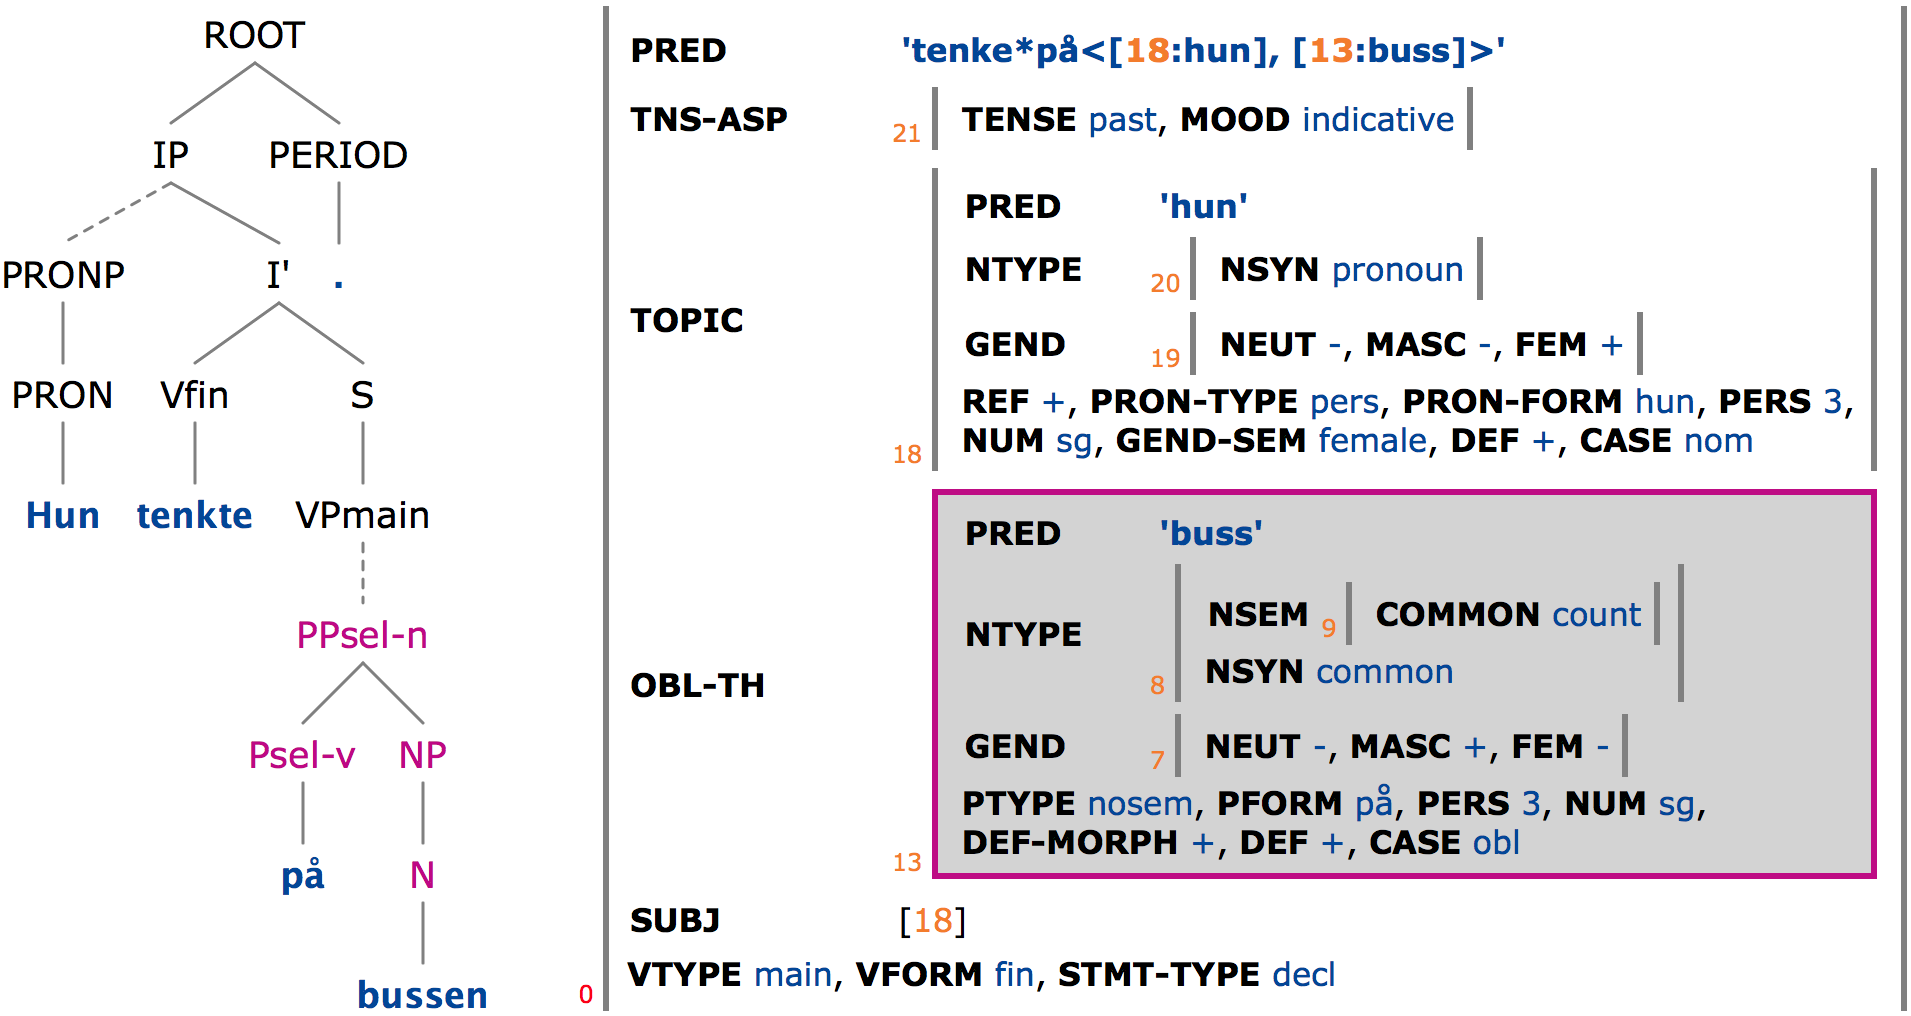
\includegraphics[width=\textwidth]{figures/selprepcons.png}
  \caption{C- and f-structure for example (\ref{dyv:ex:mweiness:tenkepå})}
  \label{dyv:fig:mweiness:selprepcons}
\end{figure}

In the c-structure \textit{på bussen} forms a prepositional \isi{phrase} PPsel-n, marked as selected by ``sel-n'' in the node label.
This analysis captures the fact that the selected preposition \textit{på} can only occur before the object, and that the preposition and its complement behave as one constituent with respect to movement, as in the topicalized version \textit{På bussen tenkte hun ofte} `The bus she was often thinking of'.
The preposition does not provide its own predicate in the f-structure, but is analyzed as incorporated in the predicate expressed by the verb to form the predicate name `tenke*på'.
In predicate names the symbol ``*'' is used to signal such combinations of a lexical predicate with a selected particle or preposition.
The complement of the preposition, \textit{bussen}, fills the function OBL-TH -- oblique-theta -- as an argument of this predicate, i.e., an oblique argument expressing a theta role.

The \isi{lexical entry} for \textit{tenke} is associated with the relevant frame through an invocation of the \isi{template} describing this class of constructions.
The relevant part of the \isi{lexical entry} for \textit{tenke} is shown in  (\ref{dyv:ex:mweiness:tenke-lex}).

\eabox{\label{dyv:ex:mweiness:tenke-lex}
{\small 
\begin{tabular}{ll}
tenke V & \{ \enspace [ ... ]\\
& | \enspace @(V-SUBJ-POBJ tenke på)\\
& | \enspace [ ... ] \enspace \}
\end{tabular}}}

The invocation of the \isi{template} V-SUBJ-POBJ has two parameters, the predicate name for the verb \textit{tenke} and the form of the selected preposition \textit{på}.
In (\ref{dyv:ex:mweiness:tenke-template}) part of the \isi{template} is shown (other parts of this \isi{template} for handling passive and other modifications are discussed in Section~\ref{dyv:sec:mweiness:variation}).

\ea\label{dyv:ex:mweiness:tenke-template}
{\small 
V-SUBJ-POBJ (P prp) =\\
\hspace{2em} @(CONCAT P `* prp \%FN)\\
\hspace{2em}  ($\uparrow$ PRED)=`\%FN<($\uparrow$ SUBJ)($\uparrow$ OBL-TH)>'\\
\hspace{2em}  ($\uparrow$ OBL-TH CHECK P-SELFORM)=prp
}
\z

The \isi{template} invokes another \isi{template} CONCAT, which concatenates the pre\-dicate name P and the preposition form \emph{prp} as the value of the variable \%FN.
In this example the result is the predicate name `tenke*på', which is then included in the value of PRED.
The last line assigns the value of \emph{prp} (\textit{på} in the example) as the value of the attribute P-SELFORM under the OBL-TH argument.
This feature is checked by the syntactic rule which introduces the selected PP, ensuring that only the preposition selected by the verb is accepted.

%The criterion for assigning a construction to the selected preposition type rather that the particle construction type is the restriction of the preposition to occur only before an object occurring in the verb \isi{phrase}.
%There is a set of cases where this criterion is not totally satisfactory: cases where the particle/preposition receives stress and does not clearly form a constituent with the object, but is still restricted to occurring before it.
%Such cases are analyzed as involving selected prepositions, in accordance with the criterion.
%An example is \textit{daske til} = `slap' in a treebank sentence like (\ref{dyv:ex:mweiness:dasketil}).

%\ea\label{dyv:ex:mweiness:dasketil}
%\gll Elise dasket til ham. \\
%     Elise slap.\textsc{pst} to him \\
%\glt `Elise slapped him'
%\z

%This leads to a slight overgeneration since the \isi{grammar} will accept the ungrammatical topicalization of \textit{til ham}: \textit{*Til ham dasket Elise}.
%However, we consider that an acceptable price to pay to avoid further complication of the \isi{grammar} and lexicon.

\subsubsection{Verb-particle constructions}\label{dyv:sec:mweiness:prtverbs}

Verb-particle constructions consist of a verb and a selected particle in the form of an adverb or an intransitively used preposition; in NorGram such elements are classified as PRT in the c-structure.
The verb and the particle express an idiosyncratic meaning.
As in \ili{English}, \isi{verb-particle constructions} in \ili{Norwegian} can have the particle either before or after an object, and obligatorily after if the object is pronominal; cf. \cite[276]{baldwin10}.
The analysis is illustrated in Figures~\ref{dyv:fig:mweiness:particlecons-c} and~\ref{dyv:fig:mweiness:particlecons-f} for the sentence in (\ref{dyv:ex:mweiness:skriveopp}).

\ea\label{dyv:ex:mweiness:skriveopp}
\gll Han \textbf{skrev} \textbf{opp} nummeret. \\
     he wrote up {the number}\\
\glt `He wrote down the number.'
\z

%\ea\label{dyv:ex:mweiness:skriveopp}
%\gll Han \textbf{skrev} \textbf{opp} nummeret. \\
%     he wrote up number.\textsc{def}.\textsc{sg}\\
%\glt `He wrote up the number.'
%\z

\begin{figure}
  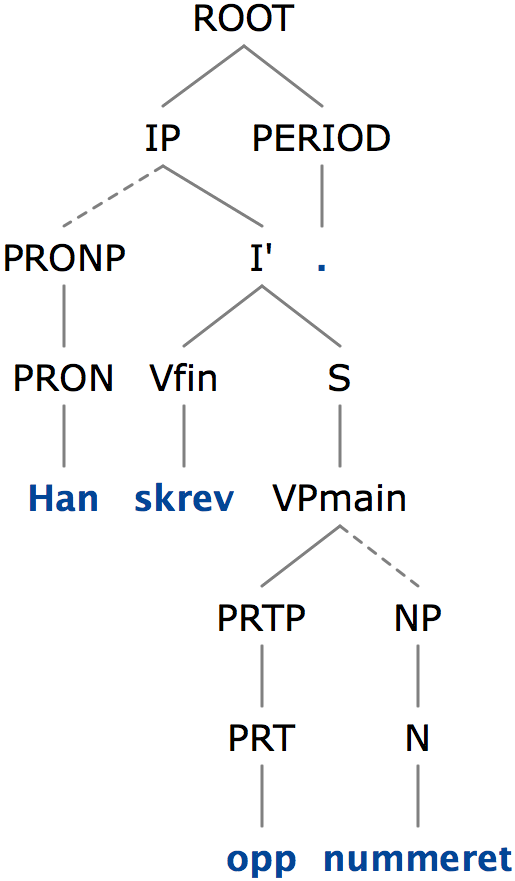
\includegraphics[width=0.27\textwidth]{figures/particlecons-c.png}
  \caption{C-structure for example (\ref{dyv:ex:mweiness:skriveopp})}
  \label{dyv:fig:mweiness:particlecons-c}
\end{figure}

\begin{figure}
  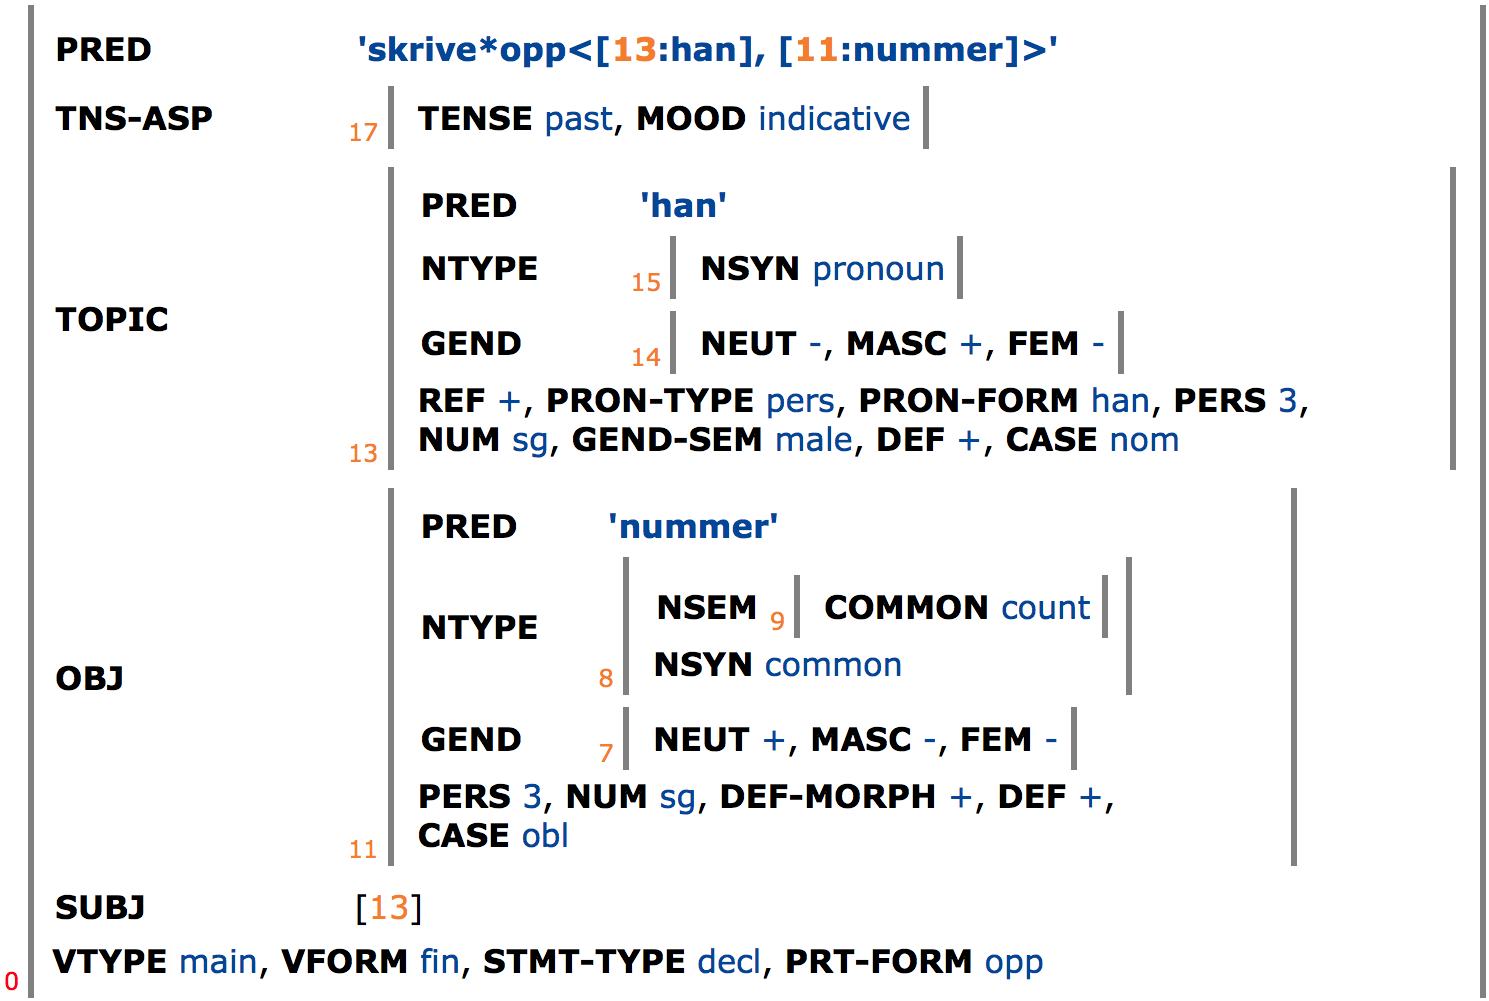
\includegraphics[width=0.75\textwidth]{figures/particlecons-f.png}
  \caption{F-structure for example (\ref{dyv:ex:mweiness:skriveopp})}
  \label{dyv:fig:mweiness:particlecons-f}
\end{figure}

%\begin{figure}
%  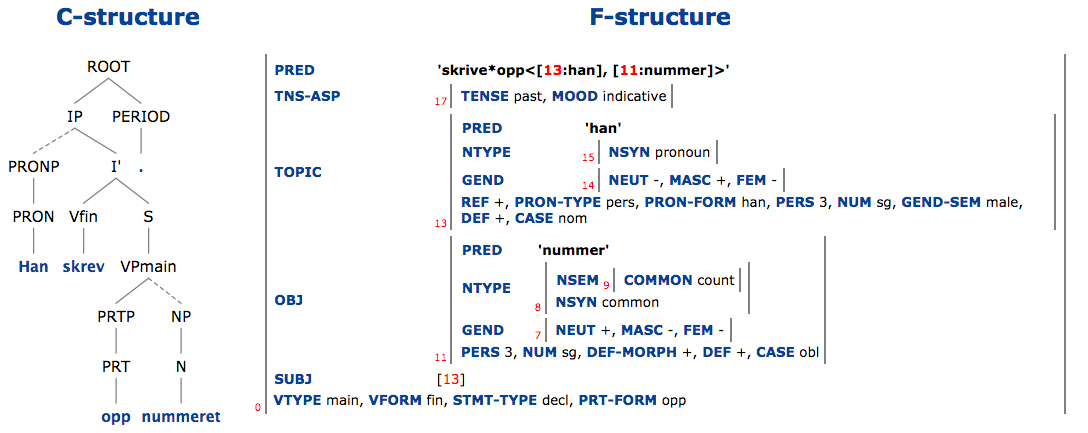
\includegraphics[width=\textwidth]{figures/particlecons.png}
%  \caption{C- and f-structure for example (\ref{dyv:ex:mweiness:skriveopp})}
%  \label{dyv:fig:mweiness:particlecons}
%\end{figure}

In the c-structure the particle PRT is a separate constituent which may also occur after the NP under VPmain.
In the f-structure the verb and the particle are analyzed as forming one predicate `skrive*opp', and the particle also provides a value to the feature PRT-FORM.

As in the case of selected prepositions, the \isi{lexical entry} for \textit{skrive} is associated with the relevant frame through an invocation of the \isi{template} describing this class of constructions.
Part of the \isi{lexical entry} for \textit{skrive} is shown in  (\ref{dyv:ex:mweiness:skrive-lex}).

\eabox{\label{dyv:ex:mweiness:skrive-lex}
{\small 
\begin{tabular}{ll}
skrive V & \{ \enspace [ ... ]\\
& | \enspace @(V-SUBJ-PRT-OBJ skrive opp)\\
& | \enspace [ ... ] \enspace \}
\end{tabular}}}

Part of the invoked \isi{template} V-SUBJ-PRT-OBJ is shown in  (\ref{dyv:ex:mweiness:skrive-template}).

\ea\label{dyv:ex:mweiness:skrive-template}
{\small 
V-SUBJ-PRT-OBJ (P prt) =\\
\hspace{2em} @(CONCAT P `* prt \%FN)\\
\hspace{2em}  ($\uparrow$ PRED)=`\%FN<($\uparrow$ SUBJ)($\uparrow$ OBJ)>'\\
\hspace{2em}  ($\uparrow$ CHECK PRT-VERB)=+\\
\hspace{2em}  ($\uparrow$ PRT-FORM)=c prt
}
\z

The CONCAT \isi{template} functions as in the \isi{template} (\ref{dyv:ex:mweiness:tenke-template}), yielding the  predicate name `skrive*opp' as the value of PRED.
The second last line assigns the value ``+'' to the path CHECK PRT-VERB, a feature which is checked by the syntactic rule introducing the particle PRT; see the VPmain rule in (\ref{dyv:ex:mweiness:rule3}) below.
The last line is a constraining equation\footnote{This concept is explained in connection with example (\ref{dyv:ex:mweiness:defrestriction}) above.} which checks that the value of the feature PRT-FORM, which is introduced in the sentence by the particle, is the value of prt, i.e. \emph{opp} in the \isi{template} invocation in (\ref{dyv:ex:mweiness:skrive-lex}).

\subsubsection{Verb-particle constructions with selected prepositions}\label{dyv:sec:mweiness:prtprepverbs}

The preceding sections have shown how \isi{prepositional verbs} and \isi{verb-particle constructions} are analyzed.
Phrasal verbs also allow both selected prepositions and particles in the same MWE.
An example involving both, in addition to a reflexive object, is provided in the treebank example in (\ref{dyv:ex:mweiness:sette-seg-inn-i}).
The analysis of (\ref{dyv:ex:mweiness:sette-seg-inn-i}) is shown in Figures~\ref{dyv:fig:mweiness:sette-seg-inn-i-c} and~\ref{dyv:fig:mweiness:sette-seg-inn-i-f}.

\ea\label{dyv:ex:mweiness:sette-seg-inn-i}
\gll Vi har et så enormt stort område å \textbf{sette} \textbf{oss} \textbf{inn} \textbf{i}.\\
     we have a such enormously large area to set us in into\\
\glt `We have such an enormously large area to immerse ourselves in.'
\z

\begin{figure}
  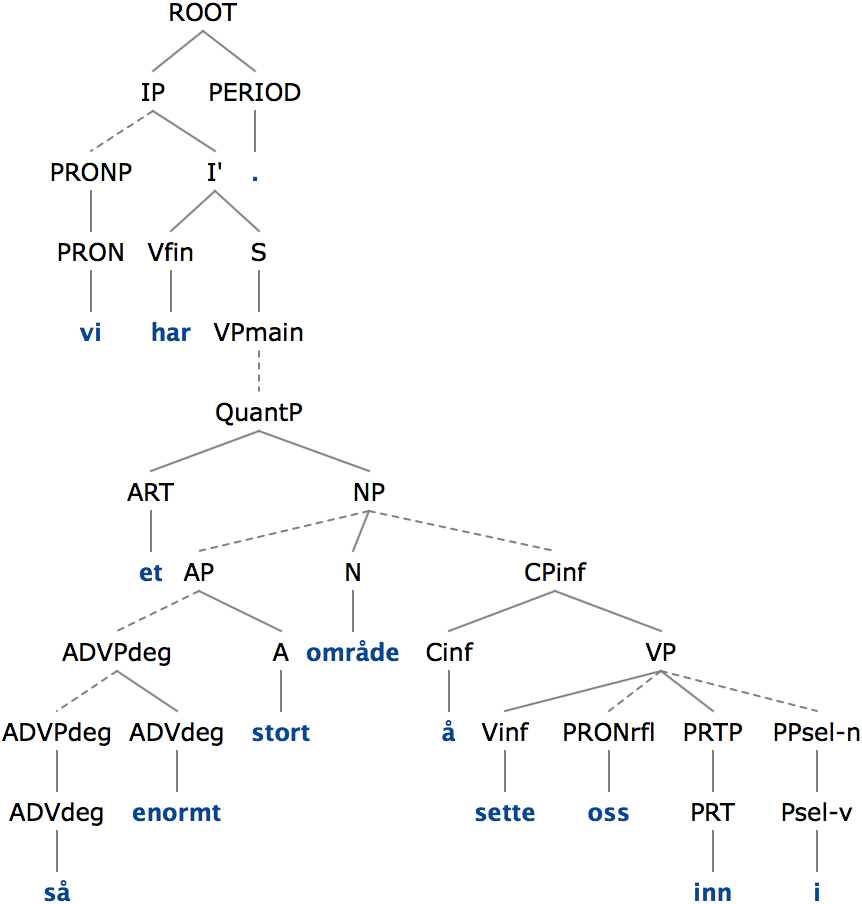
\includegraphics[height=.47\textheight]{figures/sette-seg-inn-i-c.png}
  \caption{The c-structure of sentence (\ref{dyv:ex:mweiness:sette-seg-inn-i})}
  \label{dyv:fig:mweiness:sette-seg-inn-i-c}
\end{figure}

\begin{figure}
  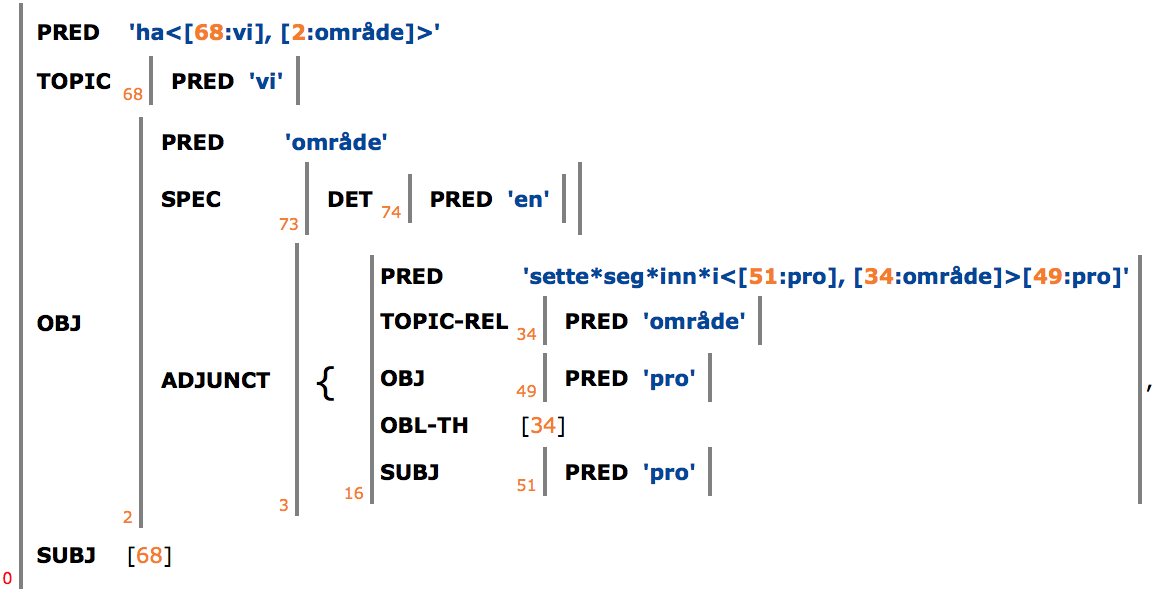
\includegraphics[width=0.9\textwidth]{figures/sette-seg-inn-i-f.png}
  \caption{Part of the simplified f-structure of sentence (\ref{dyv:ex:mweiness:sette-seg-inn-i})}
  \label{dyv:fig:mweiness:sette-seg-inn-i-f}
\end{figure}

In this example the MWE  \textit{sette oss inn i} occurs in an infinitival relative (CPinf) in an NP with the head \textit{område} `area'.
In the f-structure the infinitival relative occurs as a member of the set of adjuncts to the predicate `område', also occurring as the second argument of `sette*seg*inn*i' as its relativized argument (see Section~\ref{dyv:sec:mweiness:longdist} for the analysis of \isi{long-distance dependencies} like \isi{relativization} and topicalization).
The \isi{template} invoked by the verb \textit{sette}, V-SUBJ-OBJrefl-PRT-POBJ, provides an analysis along the lines of the templates in (\ref{dyv:ex:mweiness:tenke-template}) and (\ref{dyv:ex:mweiness:skrive-template}).

\subsection{Verbal idioms}\label{dyv:sec:mweiness:verbalidioms}

A VP idiom is a flexible MWE in which at least one predicate-bearing lexeme (such as a noun or an adjective) is selected, with possible restrictions as to number, definiteness or other morphological properties applying.
VP \isi{idioms} are handled by a specific set of templates.
For example, an idiom like \textit{holde øye med} `keep an eye on' is analyzed by means of a lexical \isi{template} covering \isi{idioms} consisting of a selected indefinite object plus a selected prepositional \isi{phrase}.
The treebank sentence in (\ref{dyv:ex:mweiness:øyemed}) is analyzed as shown in Figures~\ref{dyv:fig:mweiness:øyemed-c} and~\ref{dyv:fig:mweiness:øyemed-f}.

\ea\label{dyv:ex:mweiness:øyemed}
\gll Samtidig \textbf{holdt} han umerkelig et skarpt \textbf{øye} \textbf{med} jentungen. \\
     simultaneously kept he unnoticeably a sharp eye with {the girl child}\\
\glt `At the same time he furtively kept a close eye on the girl.'
\z

%\ea\label{dyv:ex:mweiness:øyemed}
%\gll Samtidig \textbf{holdt} han umerkelig et skarpt \textbf{øye} \textbf{med} jentungen. \\
%     simultaneously kept he unnoticably a sharp eye with girl-child.\textsc{def}.\textsc{sg}\\
%\glt `At the same time he furtively kept a sharp eye on the girl'
%\z

\begin{figure}
  \includegraphics[height=.4\textheight]{figures/øyemed-c.png}
  \caption{The c-structure of sentence (\ref{dyv:ex:mweiness:øyemed}) }
  \label{dyv:fig:mweiness:øyemed-c}
\end{figure}

\begin{figure}
  \includegraphics[height=.25\textheight]{figures/øyemed-f.png}
  \caption{The simplified f-structure of sentence (\ref{dyv:ex:mweiness:øyemed}) }
  \label{dyv:fig:mweiness:øyemed-f}
\end{figure}

The analysis of the selected prepositional \isi{phrase} \textit{med jentungen} is as described in subsection~\ref{dyv:sec:mweiness:prepverbs} for example (\ref{dyv:ex:mweiness:tenkepå}).
The selected lexeme in (\ref{dyv:ex:mweiness:øyemed}) is \textit{øye}.
In the f-structure in Figure~\ref{dyv:fig:mweiness:øyemed-f} the idiomatic meaning is represented by incorporating `øye' in the predicate name, deriving the predicate name `holde\#øye*med'. %, where we use the symbol ``\#'' to signal an idiomatic combination of this kind.
The \isi{phrase} \textit{et skarpt øye} fills the function of OBJ, but is not analyzed as a semantic argument of the sentence predicate, which appears from its position outside the angled brackets <...> surrounding the argument list.
This position signals that the constituent is syntactically subcategorized for without being a semantic argument.

The \isi{lexical entry} for \textit{holde} is associated with the VP idiom through an invocation of the idiom \isi{template} describing the relevant class of \isi{idioms}.
Part of the \isi{lexical entry} for \textit{holde} is shown in  (\ref{dyv:ex:mweiness:holde-lex}).
The \isi{template} invocation has three parameters, the predicate name for the verb \textit{holde}, the predicate of the selected noun \textit{øye},  and the form of the selected preposition \textit{med}.
Part of the \isi{template} is shown in  (\ref{dyv:ex:mweiness:holde-template}); the full \isi{template} is discussed in Section~\ref{dyv:sec:mweiness:vpidiomsyntax}.

\eabox{\label{dyv:ex:mweiness:holde-lex}
{\small 
\begin{tabular}{ll}
holde V & \{ \enspace [ ... ]\\
& | \enspace @(VPIDIOM-INDEFOBJ-POBJ holde øye med)\\
& \quad ($\uparrow$ OBJ NUM)=c sg\\
& | \enspace [ ... ] \enspace \}\\
\end{tabular}}}

\ea\label{dyv:ex:mweiness:holde-template}
{\small 
 VPIDIOM-INDEFOBJ-POBJ (P OP prp) =\\
\hspace{1.5em} @(CONCAT P `\# OP `* prp \%FN)\\
\hspace{1.5em}  ($\uparrow$  PRED)=`\%FN<($\uparrow$ SUBJ)($\uparrow$ OBL-TH)>($\uparrow$ OBJ)\\
\hspace{1.5em} ($\uparrow$ OBL-TH CHECK P-SELFORM)=prp\\
\hspace{1.5em} ($\uparrow$ OBJ PRED FN)=c OP\\
\hspace{1.5em} {\textasciitilde}($\uparrow$ OBJ DEF)=+
}
\z

In addition to the \isi{template} call, the \isi{lexical entry} in   (\ref{dyv:ex:mweiness:holde-lex}) also specifies that the selected object should be singular.
It is a matter of choice whether such information should be included in the individual \isi{lexical entry} or give rise to a distinction between more fine-grained templates.
In the \isi{template} definition in (\ref{dyv:ex:mweiness:holde-template}), OP (object predicate) is the variable for the selected noun predicate and \emph{prp} for the selected preposition.
As in the case of the \isi{template} in (\ref{dyv:ex:mweiness:skrive-template}), the \isi{template} invokes the CONCAT \isi{template} which builds the predicate name.
The second last equation requires the object to have the value of OP as its predicate (in this case `øye'), and the final equation requires the object not to be definite.
As for the equation mentioning P-SELFORM, see the explanation of the \isi{template} in (\ref{dyv:ex:mweiness:tenke-template}).

\subsection{Nonverbal flexible expressions}\label{dyv:sec:mweiness:nonverbal}

\subsubsection{Nouns with selected prepositions}\label{dyv:sec:mweiness:prepnoun}

Nouns may also form MWEs by selecting prepositional phrases as their arguments.
For example, the noun \textit{ansvar} `responsibility' may select the preposition \textit{for} `for', which can take a nominal \isi{phrase}, an infinitival, or a nominal subclause as complement, as in the treebank examples in (\ref{dyv:ex:mweiness:ansvarfor-NP})–(\ref{dyv:ex:mweiness:ansvarfor-CP}).

\ea\label{dyv:ex:mweiness:ansvarfor-NP}
\gll Hadde jeg \textbf{ansvar} \textbf{for} gutten? \\
     had I responsibility for {the boy}\\
\glt `Did I have responsibility for the boy?'
\z

%\ea\label{dyv:ex:mweiness:ansvarfor-NP}
%\gll Hadde jeg \textbf{ansvar} \textbf{for} gutten? \\
%     had I responsibility for boy.\textsc{def}.\textsc{sg}\\
%\glt `Did I have responsibility for the boy?'
%\z

\ea\label{dyv:ex:mweiness:ansvarfor-inf}
\gll Han fikk \textbf{ansvar} \textbf{for} å overta søket. \\
     he got responsibility for to take over {the search}\\
\glt `He got the responsibility for taking over the search.'
\z

%\ea\label{dyv:ex:mweiness:ansvarfor-inf}
%\gll Han fikk \textbf{ansvar} \textbf{for} å overta søket. \\
%     he got responsibility for to take over search.\textsc{def}.\textsc{sg}\\
%\glt `He got the responsibility for taking over the search.'
%\z

\ea\label{dyv:ex:mweiness:ansvarfor-CP}
\gll Jeg kan ikke ta \textbf{ansvar} \textbf{for} at det ble lekket. \\
    I can not take responsibility for that it became leaked\\
\glt `I cannot take responsibility for its having been leaked.'
\z

\begin{figure}
  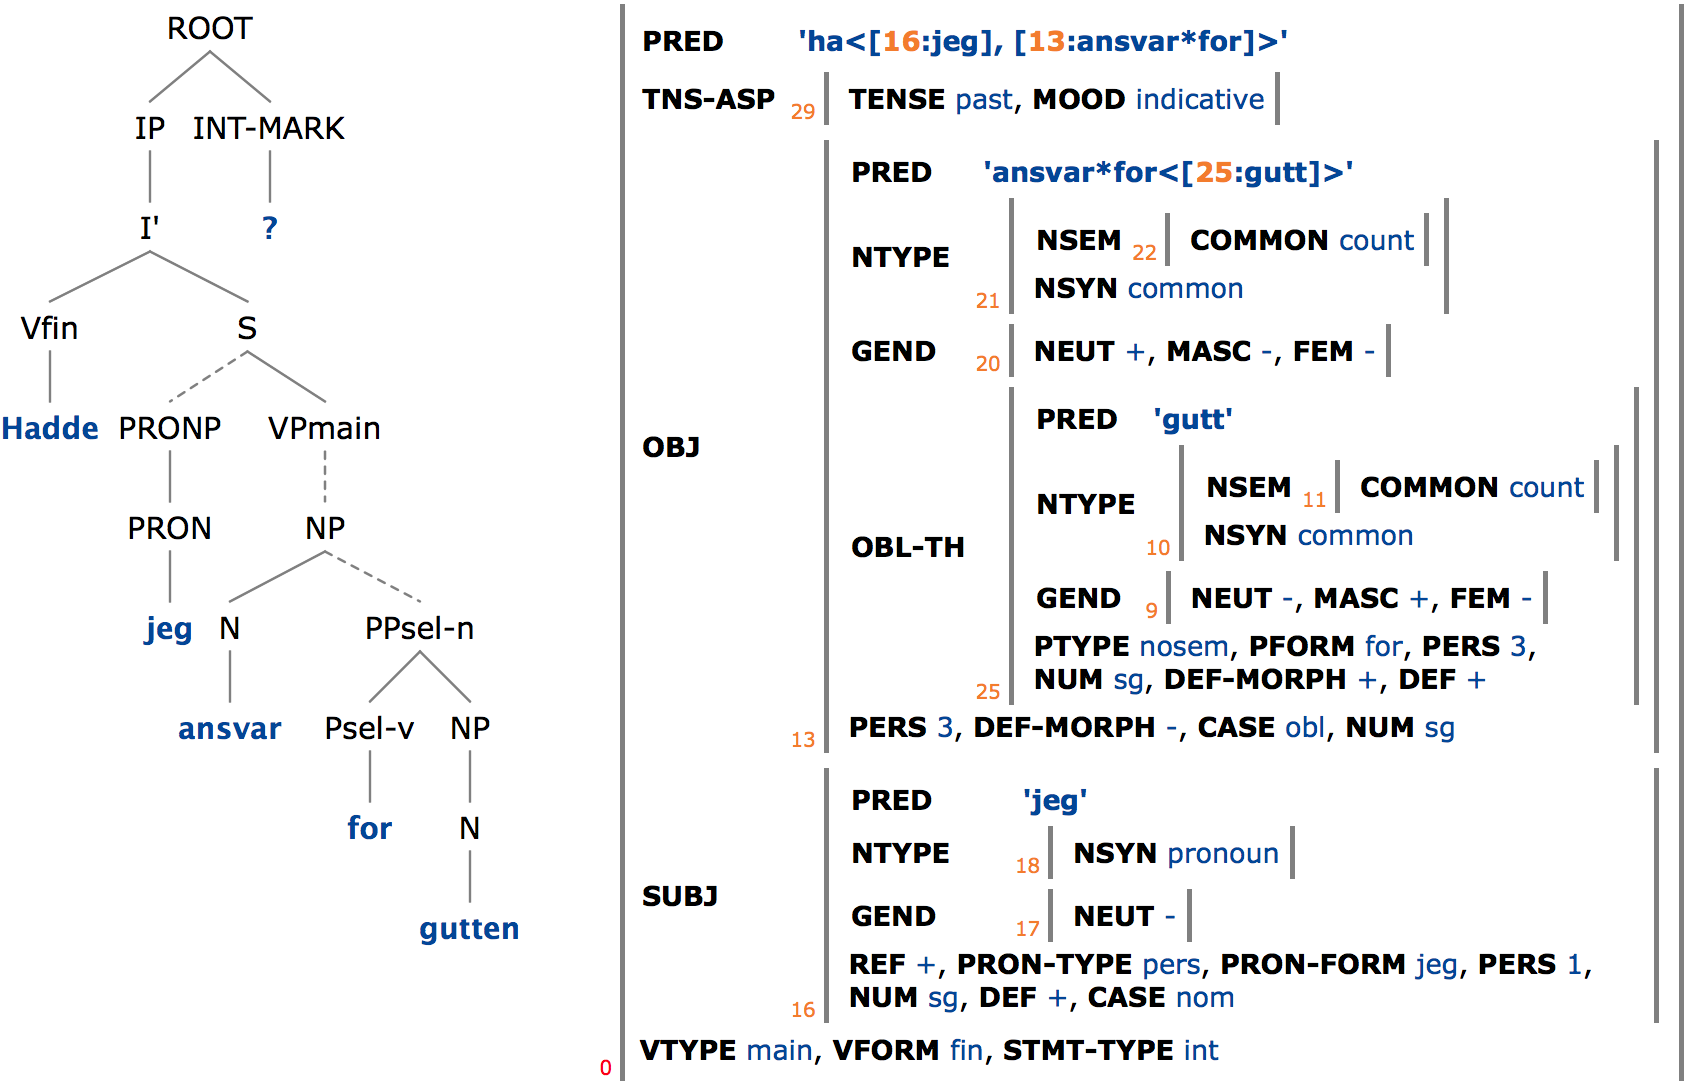
\includegraphics[width=\textwidth]{figures/ansvarfor-NP-c-f.png}
  \caption{C- and f-structure for the sentence (\ref{dyv:ex:mweiness:ansvarfor-NP}) }
  \label{dyv:fig:mweiness:ansvarfor-NP-c-f}
\end{figure}

Example (\ref{dyv:ex:mweiness:ansvarfor-NP}) is analyzed as in Figure~\ref{dyv:fig:mweiness:ansvarfor-NP-c-f}.
As in the case of \isi{prepositional verbs}, the selected preposition does not contribute a PRED of its own, but is analyzed as forming a single predicate `ansvar*for' with the noun, taking the complement of the preposition as an argument with the function OBL-TH (an oblique argument expressing a theta role).
With an infinitival or a clausal complement the syntactic function is COMP.
The \isi{lexical entry} for \textit{ansvar} in (\ref{dyv:ex:mweiness:ansvar-lex}) invokes three alternative templates for the three possible kinds of complements, in addition to its basic \isi{template} as a mass noun.

\eabox{\label{dyv:ex:mweiness:ansvar-lex}
{\small 
\begin{tabular}{ll}
ansvar N & \{ \enspace@(MASSNOUN ansvar)\\
& | \enspace @(N-POBJ ansvar for)\\
& | \enspace @(N-PINFCOMP ansvar for)\\
& | \enspace @(N-PCOMP ansvar for) \enspace \}
\end{tabular}}}

\subsubsection{Adjectives with selected prepositions}\label{dyv:sec:mweiness:prepadj}

Similarly, adjectives may select prepositional phrases as complements, for instance \textit{flink til} `clever at', as in the treebank example in (\ref{dyv:ex:mweiness:flinktil}).

\ea\label{dyv:ex:mweiness:flinktil}
\gll Hva er egentlig du \textbf{flink} \textbf{til}? \\
     what are after all you clever at\\
\glt `What are you clever at, after all?'
\z

\begin{figure}
  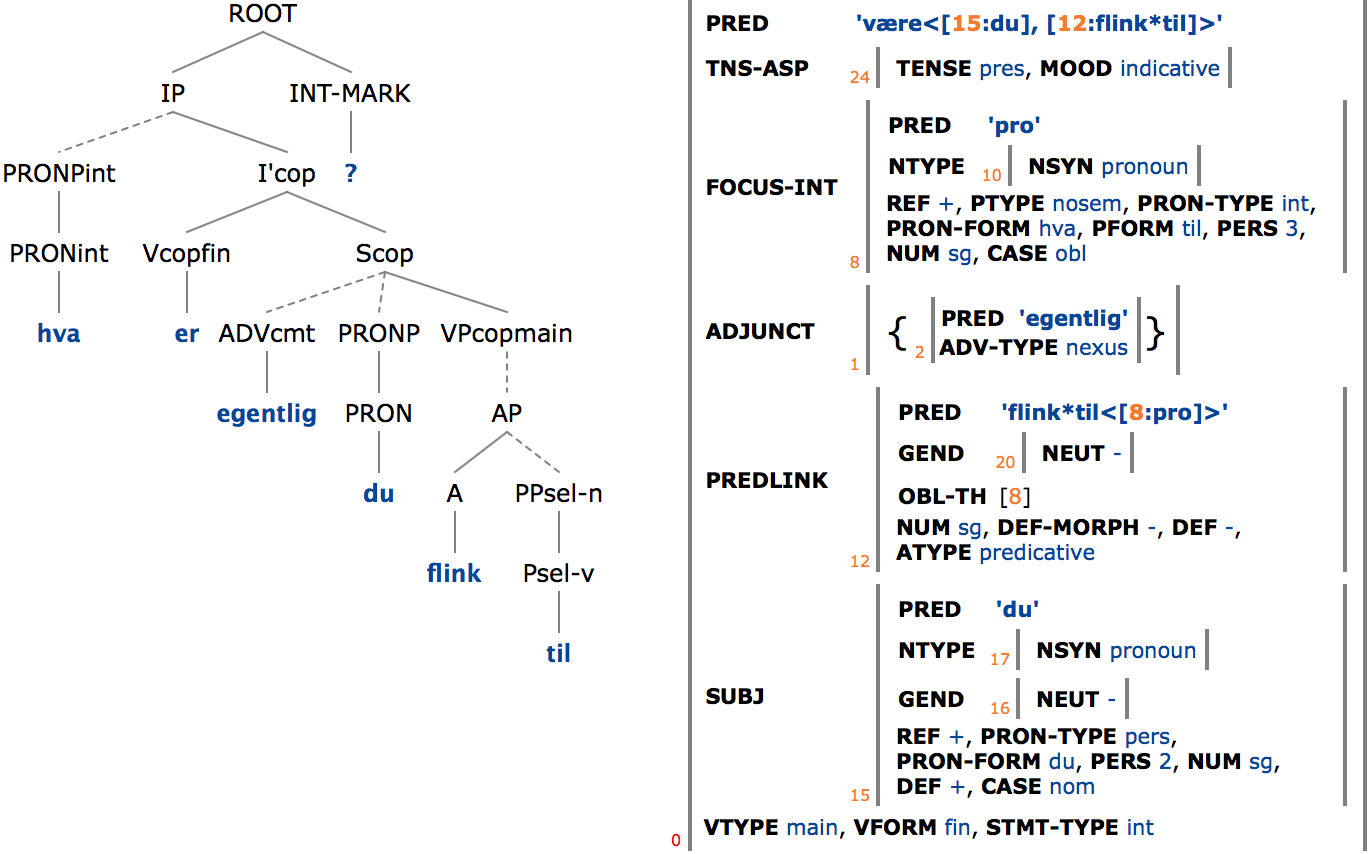
\includegraphics[width=\textwidth]{figures/flinktil-c-f.png}
  \caption{C- and f-structure for the sentence  (\ref{dyv:ex:mweiness:flinktil}) }
  \label{dyv:fig:mweiness:flinktil-c-f}
\end{figure}

Example  (\ref{dyv:ex:mweiness:flinktil}) is analyzed as in Figure~\ref{dyv:fig:mweiness:flinktil-c-f}.
In this example the complement of the selected preposition has been questioned and occurs in the f-structure as the value of FOCUS-INT, i.e., interrogative focus.
The predicative complement (PREDLINK) has the predicate `flink*til', taking the prepositional complement as its OBL-TH.
The value of OBL-TH is identical with the value of  FOCUS-INT, which is indicated by the shared index 8, resulting from the general analysis of \textit{wh}-questions in the \isi{grammar}.

\section{Representing flexibility}\label{dyv:sec:mweiness:variation}

%\subsection{Types of MWEs}
%
%NOTE-VR: Light verb constructions should be mentioned here.  Are some actually analyzed as verbal \isi{idioms}?  Check annotation guidelines for PARSEME shared task. 
%NOTE-GSL: Reflexive verbs should perhaps also be mentioned here. 
%Both reflexive verbs and LVCs are borderline cases if we assume a definition where an MWE must have at least two lexically fixed components. 
%In reflexive verbs, the variation in the reflexive is grammatical and limited; in LVCs, the variation (in the verb) is lexical and limited. 
%
%%definitions by Sag and Baldwin:
%%\citet{Sag:02}: ``idiosyncratic interpretations that cross word boundaries (or spaces)''
%%\citet{baldwin10}: ´´lexical items that: (a) can be decomposed into multiple lexemes; and (b) display lexical, syntactic, semantic, pragmatic and/or statistical \isi{idiomaticity}''

%\subsection{Syntactic `transformations'}

Flexible MWEs must be recognizable across different types of syntactic modifications which separate their parts from each other in the sentence.
Such modifications include the simple occurrence of other words between the MWE parts, \isi{long-distance dependencies} like topicalization, \isi{relativization} and \textit{wh}-question formation, presentative constructions, and various types of passive constructions.
When flexible MWEs are treated by means of \isi{LFG} templates, such modifications are automatically taken care of within the regular \isi{grammar}.
Having both a c-structure and an f-structure representation allows us to capture both the close semantic and functional association between the selecting and the selected words (in the f-structure) and their syntactic independence as different constituents (in the c-structure).
We will present the analyses of some cases.

\subsection{Intervening words}

The simplest case of syntactic modification of an MWE is when other words, typically adverbs, occur between the MWE components.
In a verb-second language like \ili{Norwegian} the sentence subject also frequently breaks up a verb \isi{phrase} MWE.
The treebank example in (\ref{dyv:ex:mweiness:trekketilbake})  illustrates the recognition of the predicate `trekke*seg*tilbake' (`withdraw', literally: `draw oneself back') across several intervening words.
The analysis is shown in Figures~\ref{dyv:fig:mweiness:trekketilbake-c} and~\ref{dyv:fig:mweiness:trekketilbake-f}. 

\ea\label{dyv:ex:mweiness:trekketilbake}
\gll Da \textbf{trekker} jeg \textbf{meg} bare stille og rolig \textbf{tilbake}.\\
     then draw I me only silently and calmly back\\
\glt `Then I simply withdraw silently and calmly.'
\z

%\ea\label{dyv:ex:mweiness:trekketilbake}
%\gll Da \textbf{trekker} jeg \textbf{meg} bare stille og rolig \textbf{tilbake}.\\
%     then draw.\textsc{prs} I me only silently and calmly back\\
%\glt `Then I simply withdraw silently and calmly.'
%\z

\begin{figure}
  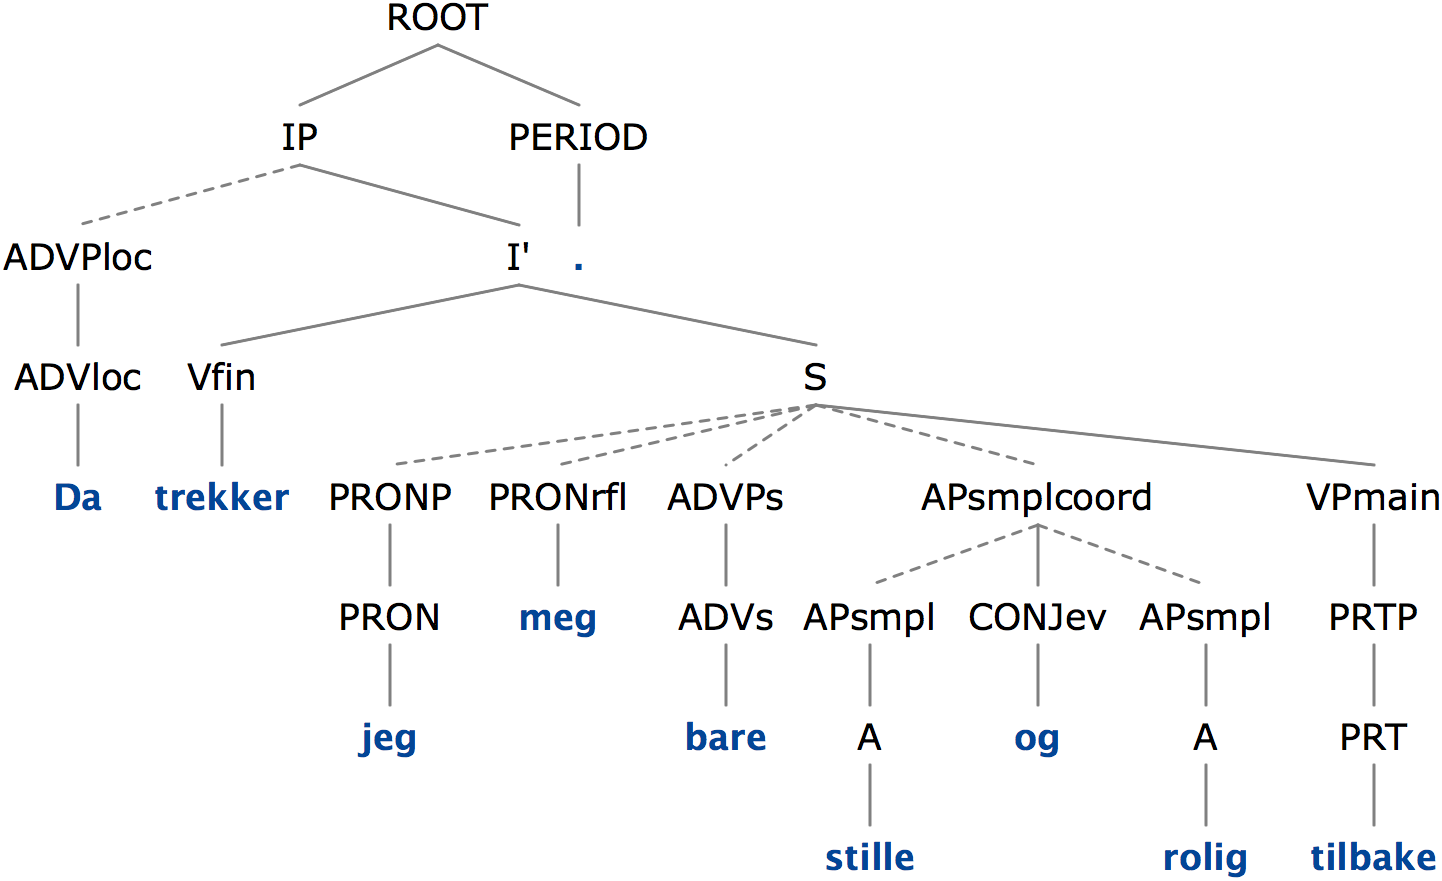
\includegraphics[height=.31\textheight]{figures/trekketilbake-c.png}
  \caption{C-structure of sentence (\ref{dyv:ex:mweiness:trekketilbake})}
  \label{dyv:fig:mweiness:trekketilbake-c}
\end{figure}

\begin{figure}
  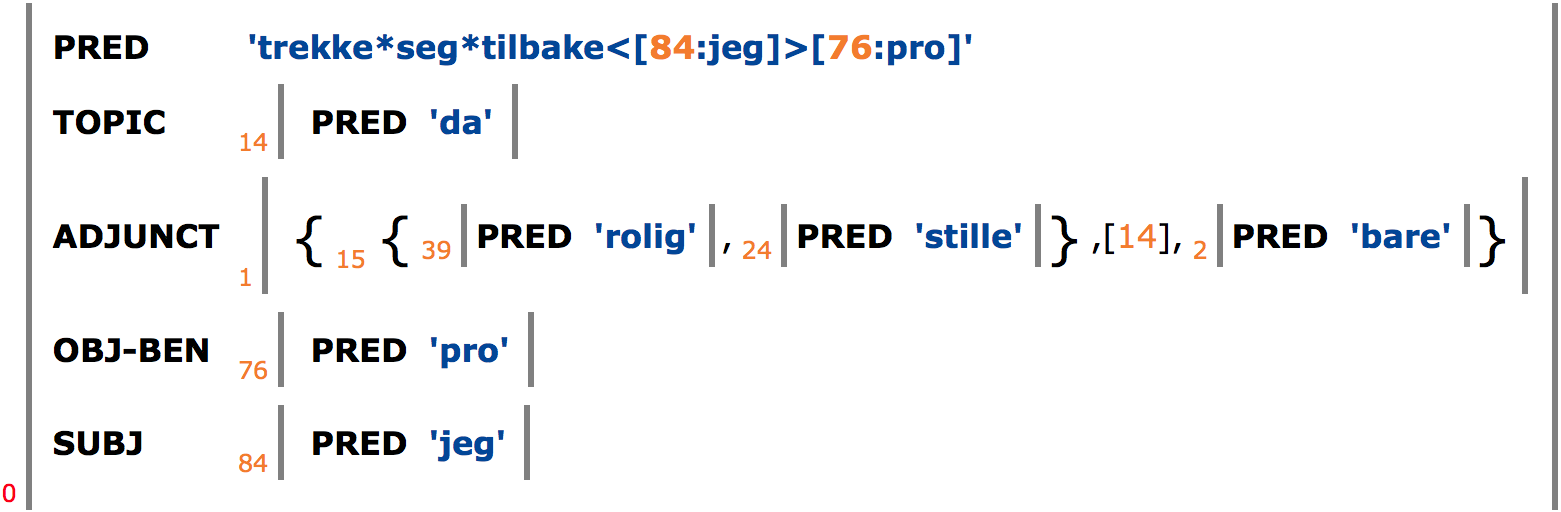
\includegraphics[height=.175\textheight]{figures/trekketilbake-f.png}
  \caption{Simplified f-structure of sentence (\ref{dyv:ex:mweiness:trekketilbake})}
  \label{dyv:fig:mweiness:trekketilbake-f}
\end{figure}

The mechanism for achieving this lies in the projection architecture of \isi{LFG}, in which different constituents in c-structure may project the same f-structure, within which dependencies may be formulated.
To illustrate we may consider the relevant fragments of the c-structure rules for I′, S and VPmain in (\ref{dyv:ex:mweiness:rule1})–(\ref{dyv:ex:mweiness:rule3}).

\eabox{\label{dyv:ex:mweiness:rule1}
{\small 
\begin{tabular}{lll}
I′ $\rightarrow$ &  Vfin: & $\uparrow$=$\downarrow$\\
 & (S: & $\uparrow$=$\downarrow$)\\\\
\end{tabular}}}

\eabox{\label{dyv:ex:mweiness:rule2}
{\small 
\begin{tabular}{lll}
S $\rightarrow$ &  (PRONP: & ($\uparrow$ SUBJ)=$\downarrow$\\
& &@SUBJCASE)\\
& [...]\\
& (PRONrfl: & \{ \enspace ($\uparrow$ OBJ-BEN)=$\downarrow$\\
& & | \enspace ($\uparrow$ OBJ)=$\downarrow$ \enspace \}) \\
& [...]\\
 & (ADVPs+: & $\downarrow$ ∈ ($\uparrow$ ADJUNCT))\\
& [...]\\
& (APsmpl:  & $\downarrow$ ∈ ($\uparrow$ ADJUNCT))\\
& [...]\\
 & (VPmain: & $\uparrow$=$\downarrow$)\\
& [...]\\\\
\end{tabular}}}

\eabox{\label{dyv:ex:mweiness:rule3}
{\small 
\begin{tabular}{lll}
VPmain $\rightarrow$ & [...]\\
& (PRTP: & $\uparrow$=$\downarrow$\\
& & ($\uparrow$ CHECK PRT-VERB)=c +)\\
& [...]\\\\
\end{tabular}}}


%\eabox{\label{dyv:ex:mweiness:rules}
%\begin{tabular}{lll}
%I' $\rightarrow$ &  Vfin: & $\uparrow$=$\downarrow$\\
% & (S: & $\uparrow$=$\downarrow$)\\\\
%\end{tabular}
%
%\begin{tabular}{lll}
%S $\rightarrow$ &  (PRONP: & ($\uparrow$ SUBJ)=$\downarrow$\\
%& &@SUBJCASE\\
%& [...]\\
%& (PRONrfl: & \{ \enspace ($\uparrow$ OBJ-BEN)=$\downarrow$\\
%& & | \enspace ($\uparrow$ OBJ)=$\downarrow$ \enspace \} \\
%& [...]\\
% & (ADVPs+: & $\downarrow$ ∈ ($\uparrow$ ADJUNCT))\\
%& [...]\\
%& (APsmpl:  & $\downarrow$ ∈ ($\uparrow$ ADJUNCT))\\
%& [...]\\
% & (VPmain: & $\uparrow$=$\downarrow$)\\
%& [...]\\\\
%\end{tabular}
%
%\begin{tabular}{lll}
%VPmain $\rightarrow$ & [...]\\
%& (PRTP: & $\uparrow$=$\downarrow$\\
%& & ($\uparrow$ CHECK PRT-VERB)=c +)\\
%& [...]\\\\
%\end{tabular}}

As explained in Section~\ref{dyv:sec:mweiness:LFG}, the equation $\uparrow$=$\downarrow$ annotated to a rule daughter means that the rule daughter and its mother will project the same f-structure.
Thus it can be seen that the Vfin daughter of I′ (the verb) and the PRTP daughter of VPmain (the particle) will project the same f-structure.

A particle verb presupposes the presence of the required particle in the sentence, and a particle presupposes the presence of a particle verb.
This mutual dependency is captured through two features, one feature PRT-VERB=+, carried by the verb and required by the rule introducing the particle, and, conversely, one feature PRT-FORM, carried by the particle and required by the verb to have the appropriate value.
Thus, the \isi{constraint} equation annotated to PRTP, ($\uparrow$ CHECK PRT-VERB)=c +, demanding that its f-structure should have a feature PRT-VERB=+ (i.e., that the verb should be a particle verb), will be satisfied if the finite verb has contributed such a feature to this common f-structure.
A similar \isi{constraint} equation associated with the verb, (($\uparrow$ PRT-FORM)=c prt in (\ref{dyv:ex:mweiness:trekke-template}) below), ensures that the particle has the form required by the verb.

The \isi{lexical entry} for \textit{trekke} is associated with the relevant frame through an invocation of the \isi{template} for reflexive \isi{verb-particle constructions}.
Part of the \isi{lexical entry} for \textit{trekke} is shown in  (\ref{dyv:ex:mweiness:trekke-lex}).
The \isi{template} has the form shown in  (\ref{dyv:ex:mweiness:trekke-template}).

\eabox{\label{dyv:ex:mweiness:trekke-lex}
{\small 
\begin{tabular}{ll}
trekke V & \{ \enspace [ ... ]\\
& | \enspace @(V-SUBJ-OBJrefl-PRT trekke tilbake)\\
& | \enspace [ ... ] \enspace \}\\
\end{tabular}}}

\ea\label{dyv:ex:mweiness:trekke-template}
{\small 
V-SUBJ-OBJrefl-PRT (P prt) =\\%[.5em]
\hspace{1.5em} @(CONCAT P `* seg `* prt  \%FN)\\%[.5em]
\hspace{1.5em}  \{ \enspace ($\uparrow$  PRED)=`\%FN<($\uparrow$ SUBJ)>($\uparrow$ OBJ-BEN)'\\%[.5em]
\hspace{1.5em} | \enspace ($\uparrow$  PRED)=`\%FN<$\uparrow$ OBJ)>($\uparrow$  OBJ-BEN)($\uparrow$ SUBJ)'\\%[.5em]
\hspace{1.5em} \quad ($\uparrow$ PRESENTATIVE)=+\\%[.5em]
\hspace{1.5em} \quad ($\uparrow$ SUBJ PRON-TYPE)=c expl\\%[.5em]
\hspace{1.5em} \quad ¬ ($\uparrow$ OBJ DEF)=+ \enspace \}\\%[.5em]
\hspace{1.5em} @(REFLEXIVE OBJ-BEN)\\%[.5em]
\hspace{1.5em} ($\uparrow$ CHECK PRT-VRB)=+\\%[.5em]
\hspace{1.5em} ($\uparrow$ PRT-FORM)=c prt\\%[.5em]
\hspace{1.5em} ¬ ($\uparrow$ PASSIVE)=+
}
\z

The \isi{template} CONCAT constructs the predicate name `trekke*seg*tilbake' as the value of PRED.
The reflexive occurring with reflexive verbs is analyzed as OBJ-BEN (indirect object).
The reason for this is that there will be a direct object in the alternative presentative construction with an expletive \textit{det} subject, such as \textit{Det trekker seg tilbake store styrker} `There are big forces withdrawing', in which \textit{store styrker} occurs as a syntactic object (OBJ); there can only be one OBJ.
The presentative construction is described as the second alternative in the disjunction \{...|...\} in the \isi{template}.
The reflexive, like the expletive subject, is analyzed as a non-argument, which appears from the fact that it is placed outside the argument list enclosed by <...> in the value of PRED.
The features PRT-VRB and PRT-FORM are explained in the discussion of the \isi{template} in (\ref{dyv:ex:mweiness:skrive-template}).

\subsection{Long-distance dependencies}\label{dyv:sec:mweiness:longdist}

Long-distance dependencies involve syntactic dependencies across an arbitrary number of clause boundaries and comprise topicalization by fronting, relative clauses and \textit{wh}-questions.
Such dependencies are handled in the f-structure by means of a special type of equations using regular expressions to specify a set of alternative attribute paths into the f-structure.
The term for this mechanism is \emph{functional uncertainty}.
The rule in (\ref{dyv:ex:mweiness:furule}) shows a simplified version of the functional uncertainty equation handling the dependency between the topic and some embedded gap further down in the structure.

\eabox{\label{dyv:ex:mweiness:furule}
  {\small
\begin{tabular}{lll}
IP $\rightarrow$ &  XP: & ($\uparrow$ TOPIC)=$\downarrow$\\
& & ($\uparrow$ \{COMP | XCOMP\}* \{SUBJ | OBJ | OBL-TH\})=$\downarrow$\\
& [ ... ]
\end{tabular}
}
}

The first equation annotated to XP in (\ref{dyv:ex:mweiness:furule}) specifies that the f-structure of the XP daughter ($\downarrow$) is the value of the attribute TOPIC of the f-structure of the IP mother ($\uparrow$).
The second equation specifies that the daughter f-structure is also the value of one of a set of alternative attribute paths.
COMP and XCOMP are the attributes of embedded finite and non-finite clauses.
The regular expression \{COMP | XCOMP\}* describes all possible strings over the elements COMP and XCOMP (with repetitions), and the final disjunction specifies the last attribute of the string, enabling the TOPIC to be identical with an embedded SUBJ, OBJ or OBL-TH.
We may illustrate with the treebank example in (\ref{dyv:ex:mweiness:fortelleom}) of a prepositional verb \textit{fortelle om} `tell about' in a sentence where the OBL-TH, i.e., the selected prepositional \isi{phrase}, has been topicalized.

\ea\label{dyv:ex:mweiness:fortelleom}
\gll \textbf{Om} dette skal jeg \textbf{fortelle} nå.\\
     about this shall I tell now\\
\glt `This I will now tell about.'
\z

%\begin{figure}
%  \includegraphics[width=\textwidth]{figures/fortelle-om-c.png}
%  \caption{C-structure for example (\ref{dyv:ex:mweiness:fortelleom})}
%  \label{dyv:fig:mweiness:fortelle-om-c-f}
%\end{figure}
%
%\begin{figure}
%  \includegraphics[width=\textwidth]{figures/fortelle-om-f.png}
%  \caption{F-structure for example (\ref{dyv:ex:mweiness:fortelleom})}
%  \label{dyv:fig:mweiness:fortelle-om-c-f}
%\end{figure}

\begin{figure}
  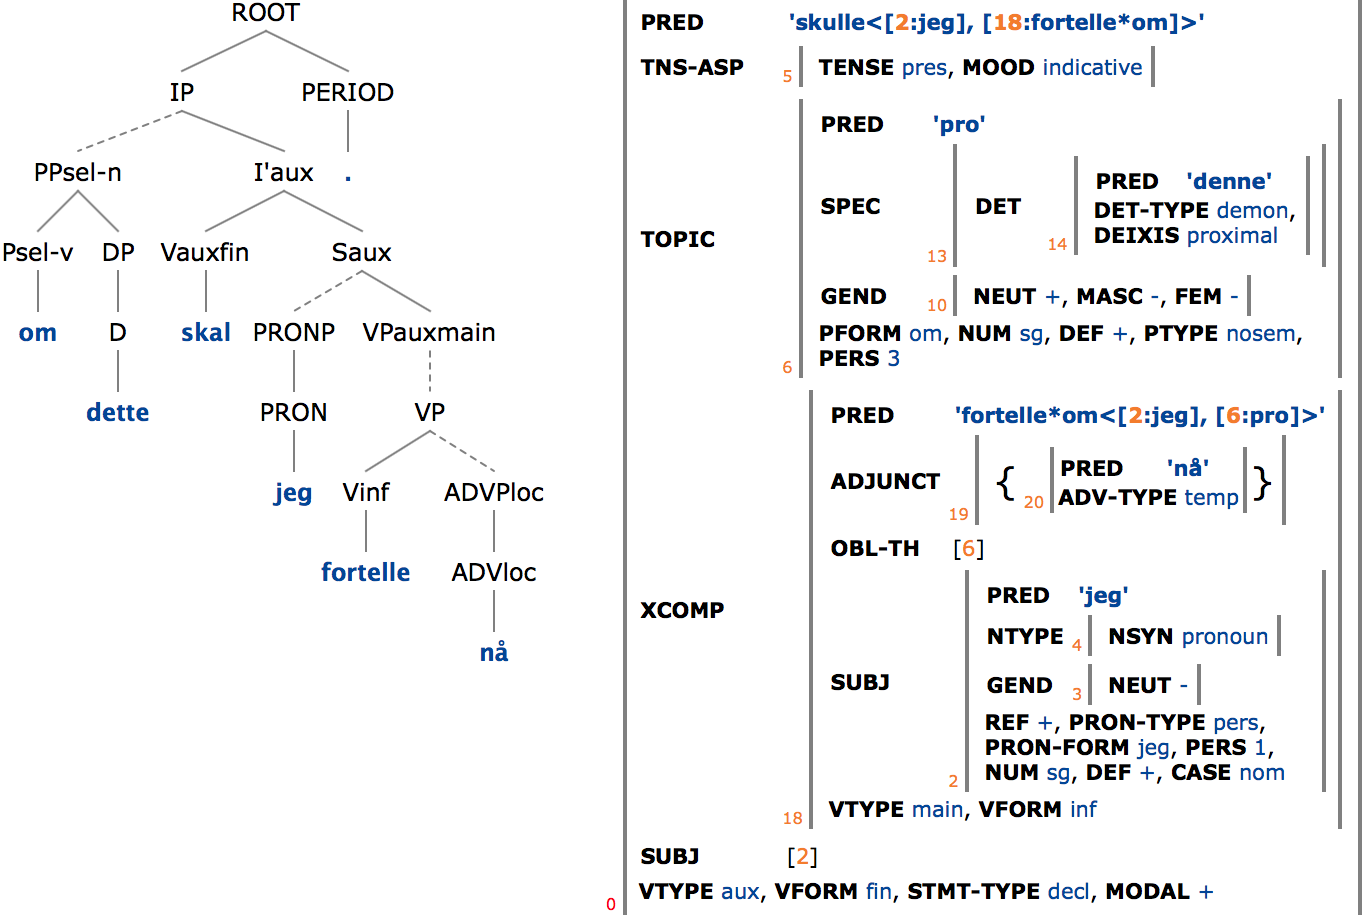
\includegraphics[width=\textwidth]{figures/fortelle-om-c-f.png}
  \caption{C- and f-structure for example (\ref{dyv:ex:mweiness:fortelleom})}
  \label{dyv:fig:mweiness:fortelle-om-c-f}
\end{figure}

The analysis of  (\ref{dyv:ex:mweiness:fortelleom}) is shown in Figure~\ref{dyv:fig:mweiness:fortelle-om-c-f}.
In the f-structure the value of TOPIC, indexed 6, is also found as the value of OBL-TH in the embedded XCOMP with `fortelle*om' as predicate.
Thus the attribute string from the set specified by the functional uncertainty equation in (\ref{dyv:ex:mweiness:furule}) for this example is ($\uparrow$ XCOMP OBL-TH).

\subsection{Passive alternations}\label{dyv:sec:mweiness:vpidiomsyntax}

Passive is another source of verbal MWE modifications, changing the syntactic functions of selected constituents.
In \isi{LFG} passive is analyzed as a lexical phenomenon modifying the value of PRED in a \isi{lexical entry} for a verb, changing the mapping between argument positions and syntactic functions.
In NorGram this is handled by passive templates invoked by the verb templates.
The full version of the VP idiom \isi{template} in (\ref{dyv:ex:mweiness:holde-template}) for \isi{idioms} like \textit{holde øye med} `keep an eye on' is shown in (\ref{dyv:ex:mweiness:holde-template-full}), where different types of passive alternations are handled.

%%\clearpage

\ea\label{dyv:ex:mweiness:holde-template-full}
{\small 
 VPIDIOM-INDEFOBJ-POBJ (P OP prp) =\\%[.5em]
\hspace{1.5em} @(CONCAT P `\# OP `* prp \%FN)\\%[.5em]
\hspace{1.5em}  \{ \enspace @(PASS-OBL-TH [($\uparrow$  PRED)=`\%FN<($\uparrow$ SUBJ)($\uparrow$ OBL-TH)>($\uparrow$ OBJ) ])\\%[.5em]
\hspace{1.5em} | \enspace \{ \enspace ($\uparrow$  PRED)=`\%FN<NULL($\uparrow$ OBL-TH)>($\uparrow$ SUBJ)($\uparrow$ OBJ)'\\%[.5em]
\hspace{1.5em} \quad | \enspace ($\uparrow$  PRED)=`\%FN<$\uparrow$ OBL-AG)($\uparrow$  OBL-TH)>($\uparrow$ SUBJ)($\uparrow$ OBJ)' \enspace \}\\%[.5em]
\hspace{1.5em} \quad ($\uparrow$ PASSIVE)=c +\\%[.5em]
\hspace{1.5em} \quad ($\uparrow$ PRESENTATIVE-TYPE)=passive\\%[.5em]
\hspace{1.5em} \quad ($\uparrow$ SUBJ PRON-TYPE)=c expl \enspace \}\\%[.5em]
\hspace{1.5em} ($\uparrow$ OBL-TH CHECK P-SELFORM)=prp\\%[.5em]
\hspace{1.5em} ($\uparrow$ OBJ PRED FN)=c OP\\%[.5em]
\hspace{1.5em} {\textasciitilde}($\uparrow$ OBJ DEF)=+
}
\z

After the second line there follows a disjunction of two alternatives.
The first alternative invokes the \isi{template} PASS-OBL-TH, taking the \isi{predicate-argument structure} as a parameter.
This \isi{template} allows the active/passive alternation whereby the OBL-TH, i.e., the complement of the selected preposition (see the discussion of example [\ref{dyv:ex:mweiness:tenkepå}]), may be the subject in a passive construction, as in the treebank example in (\ref{dyv:ex:mweiness:øyemedpass}).

\ea\label{dyv:ex:mweiness:øyemedpass}
\gll De var derimot ikke klar over at de ble \textbf{holdt} \textbf{øye} \textbf{med}. \\
     they were on the other hand not clear over that they became held eye with\\
\glt `On the other hand, they weren't aware that someone was keeping an eye on them.'
\z

The second alternative in the main disjunction describes the impersonal (presentative) passive option with an expletive subject, as in the example in (\ref{dyv:ex:mweiness:øyemedimpers}).

\ea\label{dyv:ex:mweiness:øyemedimpers}
\gll Det ble \textbf{holdt} \textbf{øye} \textbf{med} dem. \\
     it became held eye with them\\
\glt `Someone was keeping an eye on them.'
\z

The embedded disjunction of two predicate-argument structures in the fourth and fifth lines of the \isi{template} describes the possibility of including an OBL-AG, i.e., an oblique agent in a prepositional \isi{phrase} with \textit{av} `by'.
The remaining equations require the passive form of the verb and expletive type of the subject pronoun.

\section{Complementation patterns}\label{dyv:sec:mweiness:complementation}

Verbal MWEs in \ili{Norwegian} show considerable variation in terms of subcategorizational properties. 
Like simple verbs, MWEs can have transitivity shifts, take different types of arguments, and take different combinations of arguments. 
The verb-particle construction \emph{si opp}, for instance, has both an intransitive reading, as in (\ref{dyv:ex:mweiness:transitivity-a}), and a transitive reading, as in (\ref{dyv:ex:mweiness:transitivity-b}) and (\ref{dyv:ex:mweiness:transitivity-c}).
While the shift in transitivity does not significantly affect the semantics of the expression in (\ref{dyv:ex:mweiness:transitivity-b}), the shift in (\ref{dyv:ex:mweiness:transitivity-c}) leads to a change in meaning.  

\ea \label{dyv:ex:mweiness:transitivity-a} \gll 150 befal \textbf{sier} \textbf{opp}. \\ 
     150 officers say up\\
\glt `150 officers resign.' \\ 
\z

\ea \label{dyv:ex:mweiness:transitivity-b} \gll Hun \textbf{sa} \textbf{opp} jobben. \\
     she said up {the job} \\
\glt `She resigned from her job.' \\
\z

\ea \label{dyv:ex:mweiness:transitivity-c} \gll Man må \textbf{si} \textbf{opp} sjefen for Statkraft. \\
      one must say up {the boss} for Statkraft \\
\glt `The head of Statkraft must be fired.' 
\z

More precisely, the theme object that is implicit in the intransitive usage in (\ref{dyv:ex:mweiness:transitivity-a}) is explicit in (\ref{dyv:ex:mweiness:transitivity-b}), while in (\ref{dyv:ex:mweiness:transitivity-c}) the object has the semantic role of experiencer instead of theme.
The frames V-SUBJ-PRT and V-SUBJ-PRT-OBJ represent the intransitive and the transitive usages of \emph{si opp}.
NorGram, being mainly a syntactic framework, has one frame for both transitive readings, leaving semantic roles underspecified. 

Most of the \isi{verbal MWEs} in NorGram are \isi{phrasal verbs} or VP \isi{idioms}.
Such MWEs have free subjects, so that any argument variation is in the complements.\footnote{The exception to free subjects in VP \isi{idioms} is expressions with the expletive subject \emph{det} `it'. However, this type of argument variation is analyzed as a grammatical rather than a lexical selection of the subject and is thus not considered here.}
The lexical entries display a wide range of complementation patterns, one type being MWEs where the verb selects all of its complements. 
Table~\ref{dyv:tab:mweiness:selected} presents types of VP \isi{idioms} in NorGram with only selected complements. 
In \isi{idioms} where the verb subcategorizes for only one selected complement, the selected element is either a nominal (O), a prepositional ([P + O]) or a predicative (PC) complement. 
There is also a type of VP idiom with two selected complements (O~+~PRT).

\begin{table}
  \begin{tabular}{llll}
    \lsptoprule
    pattern & example & lit. translation & id. translation\\
    \midrule
    V + O & \emph{slå følge} &  `beat company' &  `accompany' \\
    & \emph{slå leir} & `beat camp' &  `camp' \\
    & \emph{ta feil} & `take wrong' & `be wrong'  \\
    & \emph{ta fyr} & `take fire' &  `catch fire' \\ \hline
    V + [P + O] & \emph{gå i oppløsning} & `go in dissolution' & `dissolve' \\ 
    & \emph{komme for en dag} & `come for a day' & `be revealed' \\     
    & \emph{løfte i flokk} & `lift in flock' & `join forces' \\
    & \emph{legge på svøm} & `lay on swim' &  `start swimming' \\ \hline
    V + PC & \emph{stå brud} & `stand bride' & `get married' \\ \hline
    V + O + PRT & \emph{sette livet til} & `put the life to' & `lose one's life' \\
    \lspbottomrule
  \end{tabular}
  \caption{Verbal MWEs with only selected complements}
  \label{dyv:tab:mweiness:selected}
\end{table}

%Verbal MWEs with simple internal structure like the examples in Table (\ref{dyv:tab:mweiness:selected}) are particularly suitable for NLP related tasks such as MWE identification, \isi{MWE extraction} and the annotation of MWEs in corpora and \isi{treebanks}. 
%\citet{gibbs89, baldwin03, mcshane04, kay12, siyanova15} are examples of very different research making use of basic MWE structures such as V + OBJ combinations in case studies and experiments.
%Many MWEs, however, have a more complex build-up with open slots that must be filled. 
%
Most \isi{verbal MWEs} in NorGram have free complements in addition to their selected complements. 
%, and one MWE will often subcategorize for different types of free complements.
In the VP idiom \emph{legge merke til} `notice', the verb \emph{legge} `lay' selects the object \emph{merke} `mark' in the indefinite form and a prepositional complement which is either nominal, as in (\ref{dyv:ex:mweiness:leggemerketil-a}), clausal, as in (\ref{dyv:ex:mweiness:leggemerketil-b}), or an interrogative clausal complement, as in  (\ref{dyv:ex:mweiness:leggemerketil-c}), all headed by the selected preposition \emph{til} `to'.

\ea \label{dyv:ex:mweiness:leggemerketil-a}
\gll Ingen \textbf{legger} \textbf{merke} \textbf{til} mannen som står urørlig og venter. \\ % i bakgrunnen. \\
     {no one} lays mark to {the man} who stands motionless and waits \\ % in {the background} \\
\glt `No one notices the man who is standing waiting motionlessly.' % in the back'
\z

\ea \label{dyv:ex:mweiness:leggemerketil-b}
\gll Ingen \textbf{legger} \textbf{merke} \textbf{til} at mannen står urørlig og venter. \\ % i bakgrunnen. \\
     {no one} lays mark to that {the man} stands motionless and waits \\ % in {the background}\\
\glt `No one notices that the man is standing waiting motionlessly.' % in the back'
\z

\ea \label{dyv:ex:mweiness:leggemerketil-c}
\gll Ingen \textbf{legger} \textbf{merke} \textbf{til} om mannen står urørlig og venter. \\ % i bakgrunnen. \\
     {no one} lays mark to if {the man} stands motionless and waits \\ % in {the background}\\
\glt `No one notices whether the man is standing waiting motionlessly.' % in the back'
\z

%\ea\label{dyv:ex:mweiness:leggemerketil}
%\begin{xlist}
%\ex \label{dyv:ex:mweiness:leggemerketil-a}
%\gll Ingen \textbf{legger} \textbf{merke} \textbf{til} \emph{mannen som står urørlig og venter}. \\ % i bakgrunnen. \\
%     {no one} lays mark to {{the man} who stands motionless and waits} \\ % in {the background} \\
%\glt `No one notices the man who stands motionless waiting.' % in the back'
%\ex \label{dyv:ex:mweiness:leggemerketil-b}
%\gll Ingen \textbf{legger} \textbf{merke} \textbf{til} \emph{at mannen står urørlig og venter}. \\ % i bakgrunnen. \\
%     {no one} lays mark to {that {the man} stands motionless and waits} \\ % in {the background}\\
%\glt `No one notices that the man stands motionless waiting.' % in the back'
%\ex \label{dyv:ex:mweiness:leggemerketil-c}
%\gll Ingen \textbf{legger} \textbf{merke} \textbf{til} \emph{om mannen står urørlig og venter}. \\ % i bakgrunnen. \\
%     {no one} lays mark to {if {the man} stands motionless and waits} \\ % in {the background}\\
%\glt `No one notices if the man stands motionless waiting.' % in the back'
%\end{xlist}
%\z

MWEs that subcategorize for different types of complements are represented in the lexicon with one frame for each \isi{subcategorization} pattern.
In the \isi{template} invocations in (\ref{dyv:ex:mweiness:leggemerketilframes}), POBJ, PCOMP and PCOMPint represent the different types of prepositional complements that occur with \emph{legge merke til} in (\ref{dyv:ex:mweiness:leggemerketil-a}), (\ref{dyv:ex:mweiness:leggemerketil-b}), and (\ref{dyv:ex:mweiness:leggemerketil-c}), respectively.

\ea\label{dyv:ex:mweiness:leggemerketilframes}
\begin{xlist}
\ex \label{dyv:ex:mweiness:leggemerketilframes-a}@(VPIDIOM-INDEFOBJ-POBJ legge merke til) \\ 
\ex \label{dyv:ex:mweiness:leggemerketilframes-b}@(VPIDIOM-INDEFOBJ-PCOMP  legge merke til) \\
\ex \label{dyv:ex:mweiness:leggemerketilframes-c}@(VPIDIOM-INDEFOBJ-PCOMPint legge merke til) \\
\end{xlist}
\z	

%Variation in the complementation is limited for individual MWEs, as is the case for \emph{legge merke til} which have three frames in which only one of the complements varies. 
%Each MWE that is added to the lexicon thus requires a relatively low number of \isi{subcategorization} frames.
%Variation in complementation patterns is mainly due to differences between MWEs, and this is reflected in the total number of unique frames.
%For instance, there are more than 80 templates for \isi{phrasal verbs}, which may be grouped into seven main classes according to the types and number of complements (Table~\ref{dyv:tab:mweiness:phrasaltypes}).\footnote{This number does not include particles and selected prepositions in VP \isi{idioms}, cf. the numbers given in Section\ref{dyv:sec:mweiness:prtprepverbs}.} 

While Table~\ref{dyv:tab:mweiness:selected} shows different types of selected complements, examples (\ref{dyv:ex:mweiness:leggemerketil-a})-(\ref{dyv:ex:mweiness:leggemerketil-c}) illustrate how one MWE may take different types of free complements.
In both cases, we see that variation in the complementation is limited for individual MWEs.
While \emph{slå følge} `accompany', \emph{gå i oppløsning} `dissolve' and the other examples in Table~\ref{dyv:tab:mweiness:selected} all have fixed complement structures, \emph{legge merke til} `notice' has three different frames in which only one of the complements varies.
To give an impression of the variety of complementation patterns in the lexicon it is thus necessary to turn to the inventory of unique frames, reflected in the number of templates.
For instance, NorGram has more than 80 templates for \isi{phrasal verbs}; these may be grouped into seven main classes according to the types and number of complements (Table~\ref{dyv:tab:mweiness:phrasaltypes}). %\footnote{This number does not include particles and selected prepositions in VP \isi{idioms}, cf. the numbers given in Section~\ref{dyv:sec:mweiness:prtprepverbs}.} 

\begin{table}
  \begin{tabular}{l@{~}l@{~}l}
    \lsptoprule
    type & example frame & example MWE \\
    \midrule
    V + PRT & V-SUBJ-PRT & \emph{stryke med} \\
    V + PRT + 1 complement & V-SUBJ-PRT-XCOMP & \emph{få til} \\
    V + PRT + 2 complements & V-SUBJ-PRT-OBJ-OBJ & \emph{gjøre etter}\\     \hline
    V + PPsel & V-SUBJ-POBJ & \emph{advare mot} \\
    V + PPsel + 1 complement  & V-SUBJ-OBJ-PACOMP & \emph{erklære for} \\
    V + PPsel + 2 complements & V-SUBJ-OBJ-POBJ-PCOMP & \emph{vedde med på} \\ \hline
    V + PRT + PPsel & V-SUBJ-PRT-POBJ & \emph{gå med på} \\
    V + PRT + PPsel + 1 complement & V-SUBJ-PRT-OBJ-POBJ & \emph{venne av med} \\ % gjøre om til
    \lspbottomrule
  \end{tabular}
  \caption{Main types of complementation patterns in phrasal verbs in NorGram}
  \label{dyv:tab:mweiness:phrasaltypes}
\end{table}

Table~\ref{dyv:tab:mweiness:phrasaltypes} presents the different types of complementation patterns for \isi{verb-particle constructions}, \isi{prepositional verbs}, and \isi{verb-particle constructions} with selected prepositions.
The first column in the table is the pattern type, represented in terms of the main complement(s), which may be a particle (PRT), a selected prepositional \isi{phrase} (PPsel), or both, and the number of additional complements.\footnote{``Main complement'' in this context refers to the selected complement which determines the type of the overall construction, such as PRT in \isi{verb-particle constructions}.} 
%The first column in the table is the pattern type, represented in terms of the main complement (PRT, PPsel or both) and the number of additional complements.\footnote{``Main complement'' in this context refers to the selected complement which determines the type of the overall construction, such as PRT in \isi{verb-particle constructions}.} 
Examples of \isi{subcategorization} frames for each type are given in the second column using \isi{template} names.
The example MWEs, represented in the table with only their fixed components, are instances of the example frames and are discussed in more detail in (\ref{dyv:ex:mweiness:strykemed})-(\ref{dyv:ex:mweiness:venneavmed}).

 As Table~\ref{dyv:tab:mweiness:phrasaltypes} shows, \isi{verb-particle constructions} in NorGram may either be intransitive, such as \emph{stryke med} `die' in (\ref{dyv:ex:mweiness:strykemed}), or have one or two free complements, such as \emph{få noe til} `accomplish something' in (\ref{dyv:ex:mweiness:fåtil-1}) and \emph{gjøre noen noe etter} `repeat something after someone' in (\ref{dyv:ex:mweiness:gjøreetter}).

%As Table~\ref{dyv:tab:mweiness:phrasaltypes} shows, particle-verb constructions in NorGram are either intransitive, such as \emph{stryke med} `die' in (\ref{dyv:ex:mweiness:strykemed}) which only requires a subject, transitive like \emph{få noe til} `accomplish something' in (\ref{dyv:ex:mweiness:fåtil}),  or ``ditransitive'' with two free complements such as  \emph{gjøre noen noe etter} `do someone something after'  in (\ref{dyv:ex:mweiness:gjøreetter}).
%As Table~\ref{dyv:tab:mweiness:phrasaltypes} shows, \isi{verb-particle constructions} in NorGram are either intransitive, such as \emph{stryke med} `die' in (\ref{dyv:ex:mweiness:strykemed}) which only requires a subject, or may have one or two free complements, such as \emph{få noe til} `accomplish something' in (\ref{dyv:ex:mweiness:fåtil-1}) and \emph{gjøre noen noe etter} `repeat something after someone' in (\ref{dyv:ex:mweiness:gjøreetter}).

%Og vi fortsetter å banke deg til du stryker med!»
%Treebank: nob-novel_2 version: 2016-05-17; Document: Brandstadmoen, Geir: På barndommens solbrente enger; \isi{grammar}: \ili{Norwegian} Bokmål
%Sentence #4024
\ea\label{dyv:ex:mweiness:strykemed}
\gll Og vi fortsetter å banke deg til du \textbf{stryker} \textbf{med}! \\ 
 and we continue to beat you until you stroke with \\
\glt `And we will continue to beat you until you're dead!' \\ 
\z

\ea\label{dyv:ex:mweiness:fåtil-1}
\gll Nå \textbf{fikk} han \textbf{til} å tenke igjen. \\
 now got he to to think again \\
\glt `Now he managed to think again.' \\
\z

%%Ikke mange kunne ha gjort ham noe slikt etter!
%%Treebank: nob-child version: 2016-05-17; Document: Pedersen, Erling: Hvile i grønne enger; \isi{grammar}: \ili{Norwegian} Bokmål
%%Sentence #2774
%
\ea\label{dyv:ex:mweiness:gjøreetter}
\gll Ikke mange kunne ha \textbf{gjort} ham noe slikt \textbf{etter}! \\ 
  not many could have done him something {like that} after \\
\glt `Not many people could have done what he did!' \\ 
\z


The example \emph{få noe til} in (\ref{dyv:ex:mweiness:fåtil-1}) is an instantiation of the frame V-SUBJ-PRT-XCOMP, with one free complement in the form of the infinitival complement \emph{å tenke igjen} `to think again'.  
There is one other frame for this particular MWE in the lexicon, with a nominal object instead of the infinitival complement (V-SUBJ-PRT-OBJ). 
Example (\ref{dyv:ex:mweiness:fåtil-2}) illustrates this complement structure.

%«Dette er hva du fikk til.»
%Treebank: nob-avis version: 2016-05-17; Document: Østli, Kjetil: ; \isi{grammar}: \ili{Norwegian} Bokmål
%Sentence #6
\ea\label{dyv:ex:mweiness:fåtil-2}
\gll Dette er hva du \textbf{fikk} \textbf{til}. \\ 
 this is what you got to \\
\glt `This is what you accomplished.' \\ 
\z

The lexicon also has a frame for \emph{få til} with two free complements, in the form of an object and an infinitival complement. 
The difference in the number of complements also yields a difference in meaning, as shown in (\ref{dyv:ex:mweiness:fåtil-3}). 
These should thus be considered different MWEs.

%http://clarino.uib.no/iness/lfg-sentence?treebank=nob-avis&version=2016-05-17&unique-id=3856989&solution-nr=2&session-id=241982373627117
\ea\label{dyv:ex:mweiness:fåtil-3}
\gll Hvorfor \textbf{får} vi ikke dem \textbf{til} å bli? \\
 why get we not them to to stay \\
\glt `Why can't we make them stay?' \\ 
\z

The last type of verb-particle construction in Table~\ref{dyv:tab:mweiness:phrasaltypes}, with two free complements in addition to the particle, is exemplified with the frame V-SUBJ-PRT-OBJ-OBJ.
This argument structure, illustrated in (\ref{dyv:ex:mweiness:gjøreetter}) for \emph{gjøre noen noe etter}, involves both an indirect object (OBJ-BEN), \emph{ham} `him', and a direct object (OBJ), \emph{noe slikt} `something like that' (OBJ-BEN is shortened to OBJ in the name of the \isi{template}).
%This argument structure, illustrated in (\ref{dyv:ex:mweiness:gjøreetter}) for \emph{gjøre noen noe etter}, is idiosyncratic because verbs normally do not take two objects.
%Other frames with two free complements are V-SUBJ-PRT-POBJrefl-COMPat and V-SUBJexpl-PRT-OBJ-COMP.
A second frame of this type, which is slightly more complex with a nominal object and a clausal complement (COMP) as well as an expletive subject, is V-SUBJexpl-PRT-OBJ-COMP. 
The MWE \emph{det faller noen noe inn} `something occurs to someone' in (\ref{dyv:ex:mweiness:falleinn}) is an example of this frame, literally translating into `it falls someone something in'.
Except for the expletive subject and the particle, the frame has the same arguments as V-SUBJ-OBJ-COMP for single verbs such as \emph{forklare} `explain'.
The frame is thus regular in terms of argument structure.   
%\footnote{Compare to the frame V-SUBJ-OBJ-COMP for the verb \emph{forklare} `explain'.} 
%http://clarino.uib.no/iness/lfg-sentence?treebank=nob-avis&version=2016-05-17&unique-id=3789406&solution-nr=0&session-id=241982373627117
%Det falt ikke britene inn at særlig mange hadde lyst.

\ea\label{dyv:ex:mweiness:falleinn}
\gll   Det \textbf{falt} ikke britene \textbf{inn} at særlig mange hadde lyst. \\
        it fell not {the Brits} in that particularly many had desire \\
\glt  `It did not occur to the Brits that more than a few should want to.' \\ 
\z

In contrast to \isi{verb-particle constructions} which may be intransitive, \isi{prepositional verbs} will always have a free complement, introduced by the selected preposition.
Prepositional verbs can subcategorize for exactly one prepositional \isi{phrase}, as in
\emph{advare mot noe} `warn against something' in (\ref{dyv:ex:mweiness:advaremot}), where \emph{mot segregering} `against segregation' is a PPsel. 

%Treebank: nob-avis version: 2016-05-17; Document: Stærk, Bjørn: ; \isi{grammar}: \ili{Norwegian} Bokmål
%Sentence #62: Han advarer mot segregering.
%http://clarino.uib.no/iness/lfg-sentence?treebank=nob-avis&version=2016-05-17&unique-id=3789421&solution-nr=0
\ea\label{dyv:ex:mweiness:advaremot}
\gll   Han \textbf{advarer} \textbf{mot} segregering. \\
        he warns against segregation\\
\glt  `He warns against segregation.' \\ 
\z

Similar to \isi{verb-particle constructions}, the \isi{prepositional verbs} in NorGram can take one or two complements in addition to the selected complement. 
In (\ref{dyv:ex:mweiness:erklærefor}), \emph{erklære noen for noe} `declare someone something' has one complement, the free object \emph{marken} `the mark',  in addition to the selected prepositional \isi{phrase}  \emph{for død} `for dead'. 

%Treebank: nob-fn version: 2016-05-17; Document: Spilde, Ingrid: Økonomisk oppstandelse i virtuell verden; \isi{grammar}: \ili{Norwegian} Bokmål
%Sentence #24: – Der måtte myndighetene erklære marken for død.
\ea\label{dyv:ex:mweiness:erklærefor}
\gll   Der måtte myndighetene \textbf{erklære} marken \textbf{for} død. \\
        there {had to} {the government} declare {the mark} for dead \\
\glt `There the authorities had to declare the (\ili{German}) mark dead.'\\ 
\z

%The MWE in (\ref{dyv:ex:mweiness:erklærefor}) examplifies the pattern type V + PPsel + 1 complement in Table~\ref{dyv:tab:mweiness:phrasaltypes}, and has the \isi{subcategorization} frame V-SUBJ-OBJ-PACOMP.   
The relevant frame in (\ref{dyv:ex:mweiness:erklærefor}) is V-SUBJ-OBJ-PACOMP, where PACOMP is the selected prepositional \isi{phrase}.
While PPsel is the c-structure category for constituents headed by selected prepositions and may refer to any type of prepositional complement, PACOMP is a syntactic variable that reflects the type of complement. %, cf. POBJ, PCOMP and PXCOMP in (\ref{dyv:ex:mweiness:leggemerketilframes}). 
In this case, the preposition \emph{for} takes the adjectival predicative complement \emph{død} `dead'. %\footnote{A nominal predicative complement (as in \emph{declare someone king}) would be represented with the category NCOMP in the \isi{subcategorization} frame.}

The final type of prepositional verb in Table~\ref{dyv:tab:mweiness:phrasaltypes} is illustrated in (\ref{dyv:ex:mweiness:veddemedpå}) with the MWE \emph{vedde noe med noen på noe} `bet something with someone on something'. 

\ea\label{dyv:ex:mweiness:veddemedpå}
\gll   Abrams \textbf{veddet} en sigarett \textbf{med} Browne \textbf{på} at det regnet. \\
        Abrams bet a cigarette with Brown on that it rained \\
\glt `Abrams bets a cigarette with Brown that it {was raining}.' \\ 
\z

This example is an instance of the frame V-SUBJ-OBJ-POBJ-PCOMP, which has two complements in addition to a PPsel, in this case a free object and a second PPsel.
The free object is \emph{en sigarett} `a cigarette'.
In the first PPsel, which corresponds to POBJ in the \isi{subcategorization} frame, the selected preposition \emph{med} `with' takes the nominal object \emph{Brown}. 
In the second PPsel, corresponding to PCOMP,  the preposition \emph{på} `on' takes the clausal complement \emph{at det regnet} `that it was raining'.

Like \isi{prepositional verbs}, \isi{verb-particle constructions} with selected prepositions always subcategorize for at least one free complement. 
Such constructions can have one complement, as in \emph{gå med på noe} `go along with something' in (\ref{dyv:ex:mweiness:gåmedpå}), which is an instance of the frame V-SUBJ-PRT-POBJ.
 
%Treebank: nob-avis version: 2016-05-17; Document: Melgård, Marie; Kagge, Gunnar: ; \isi{grammar}: \ili{Norwegian} Bokmål
%Sentence #27: I land som Sverige gikk fagbevegelsen med på de nye tankene.
%http://clarino.uib.no/iness/lfg-sentence?treebank=nob-avis&version=2016-05-17&unique-id=3935000&solution-nr=36
\ea\label{dyv:ex:mweiness:gåmedpå}
\gll   I land som Sverige \textbf{gikk} fagbevegelsen \textbf{med} \textbf{på} de nye tankene. \\
        in countries like Sweden went {the unions} with on the new thoughts \\
\glt `In countries like Sweden the unions went along with the new ideas.' \\
\z

In (\ref{dyv:ex:mweiness:gåmedpå}), the particle is \emph{med} `with', and the free argument  \emph{de nye tankene} `the new thoughts' is the complement of the selected preposition \emph{på} `on'.  
The prepositional complement could, however, also be clausal, as in (\ref{dyv:ex:mweiness:gåmedpå-2}), or infinitival, as in (\ref{dyv:ex:mweiness:gåmedpå-3}).
With the infinitival complement, there is a shift in meaning from `go along with'/`admit' to `agree'. 

\ea\label{dyv:ex:mweiness:gåmedpå-2}
\gll   Han vil ikke \textbf{gå} \textbf{med} \textbf{på} at hun er utpreget modig. \\
        he will not go with on that she is exceptionally brave \\
\glt `He will not admit that she is exceptionally brave.' \\
\z

\ea\label{dyv:ex:mweiness:gåmedpå-3}
\gll   Til Libbys forbauselse hadde Jerry \textbf{gått} \textbf{med} \textbf{på} å prøve. \\
        to Libby's surprise had Jerry gone with on to try \\
\glt `To Libby's surprise, Jerry had agreed to try.' \\
\z


%http://clarino.uib.no/iness/lfg-sentence?treebank=nob-avis&version=2016-05-17&unique-id=3857732&solution-nr=1&session-id=241982373627117
%– Jeg går ut fra at de var under sterkt politisk press.

%(V-SUBJ-PRT-PXCOMP ende ende opp med)
%http://clarino.uib.no/iness/lfg-sentence?treebank=nob-lbk-sa&version=2016-05-17&unique-id=4393751&solution-nr=0&session-id=241982373627117
%Jeg ville ikke ende opp med et kulehull i brystet.

Verb-particle constructions with selected prepositions may also have two free complements. 
This is the case for \emph{venne noen av med noe} `wean someone off something' in (\ref{dyv:ex:mweiness:venneavmed}).
This example, instantiating the frame V-SUBJ-PRT-OBJ-POBJ, has the particle \emph{av} `off', the free pronominal object \emph{meg} `me', and the selected prepositional object \emph{med det} `with that'.
Also here, the prepositional complement may vary.
The alternative frame is V-SUBJ-PRT-OBJ-PXCOMP, allowing an infinitival prepositional complement, but in this case yielding no difference in meaning.

%Mor klarte aldri å venne meg av med det.
%http://clarino.uib.no/iness/lfg-sentence?treebank=nob-novel_2&version=2016-05-17&unique-id=2170917&solution-nr=0
\ea\label{dyv:ex:mweiness:venneavmed}
\gll   Mor klarte aldri å \textbf{venne} meg \textbf{av} \textbf{med} det. \\
         mother managed never to accustom me off with that \\
\glt `{Mother} never managed to wean me off that habit.' \\
\z

%A slightly more complex example of this pattern is the frame V-SUBJ-PRT-POBJrefl-COMPat.
%This is the \isi{template} for MWEs with a PPsel whose complement is a reflexive object (POBJrefl), and which also takes a clausal complement starting with the subjunction \emph{at} `that' (COMPat).\footnote{In contrast, clausal complements of the type COMP do not require the subjunction.}   
%The MWE \emph{ta noe inn over seg} `realize/admit something' has this structure. 
%The literal translation is `take something in over oneself'.

The examples of complementation patterns for \isi{phrasal verbs} in NorGram show that the subcategorizational properties of MWEs can be the source of variation both at the syntactic and the semantic levels. 
We have seen that the main types of complementation patterns in Table~\ref{dyv:tab:mweiness:phrasaltypes} are shared by a number of \isi{subcategorization} frames. %, which indicates a certain variance within each type. 
Table~\ref{dyv:tab:mweiness:ppsel1comp} presents some of the frames that are variants of the type V + PPsel + 1 complement in Table~\ref{dyv:tab:mweiness:phrasaltypes} (\isi{prepositional verbs} with one free complement). 
The frames are divided into groups of MWEs that share the same or similar types of arguments, resulting in five categories of argument patterning for this type.\footnote{Several frames of this type are not listed here, including frames with expletive subjects and objects and subtypes of clausal complements.} 
%Presenting these argument types would require some elaboration and they are thus left out of this overview.}
%Subcategorization frames for new MWEs have so far been added to the lexicon under the relevant \isi{lexical entry}, ensuring that the MWE will receive an idiomatic analysis during parsing. 
While the current section provides only superficial observations about the types of MWE argument patterns in the NorGram lexicon, it seems that a more systematic study of their subcategorizational properties could provide useful information about MWE types and tokens and perhaps also new insights into the relationship between argument patterns and the semantics of MWEs.
 
\begin{table}[htbp]
  \begin{tabular}{ll}
    \lsptoprule
complementation type & subcategorization frame \\
    \midrule
free object & V-SUBJ-OBJ-PACOMP \\
and PPsel & V-SUBJ-OBJ-POBJACOMP \\
& V-SUBJ-OBJ-POBJNCOMP \\
& V-SUBJ-OBJ-POBJ \\
& V-SUBJ-OBJ-PCOMP \\
& V-SUBJ-OBJ-PCOMPinf \\
& V-SUBJ-OBJ-PCOMPint \\
& V-SUBJ-OBJ-PXCOMP \\ 
& V-SUBJ-INDOBJ-POBJ \\
%& V-SUBJ-OBJexpl-POBJ \\
& V-SUBJexpl-OBJ-POBJ \\ \hline
Reflexive object  & V-SUBJ-OBJrefl-POBJ \\
 and PPsel  & V-SUBJ-OBJrefl-PCOMP \\
& V-SUBJ-OBJrefl-PCOMPat \\
& V-SUBJ-OBJrefl-PCOMPint \\
& V-SUBJ-OBJrefl-PXCOMP \\ \hline
PPsel & V-SUBJ-POBJ-COMP \\
and free  & V-SUBJ-POBJ-XCOMP \\
nominal  & V-SUBJ-POBJ-OBL \\
complement & V-SUBJ-POBJ-OBLBEN \\ \hline
prepositional reflexive object & V-SUBJ-POBJrefl-OBJ \\
and free nominal complement & V-SUBJ-POBJrefl-COMP \\ \hline
PPsel & V-SUBJ-POBJ-PXCOMP \\
and PPsel & V-SUBJ-POBJrefl-POBJ \\ %\hline
        \lspbottomrule
  \end{tabular}
  \caption{Some variants of  V + PPsel + 1 complement}
  \label{dyv:tab:mweiness:ppsel1comp}
\end{table}
 
 %V + PPsel + 1 complement
%V-SUBJ-OBJ-PACOMP: 2
%V-SUBJ-OBJ-POBJACOMP: 9
%V-SUBJ-OBJ-POBJACOMPsubj: 1
%V-SUBJ-OBJ-POBJNCOMP: 15
%V-SUBJ-OBJ-POBJ: 124
%V-SUBJ-OBJ-PCOMP: 16
%V-SUBJ-OBJ-PCOMPinf: 3
%V-SUBJ-OBJ-PCOMPint: 4
%V-SUBJ-OBJ-PXCOMP: 43
%V-SUBJ-OBJ-PXCOMPfå: 1
%V-SUBJ-OBJ-PXCOMPobjcont: 3
%V-SUBJ-OBJ-PXCOMPsubjcont: 7
%
%V-SUBJ-OBJrefl-POBJ: 115
%V-SUBJ-OBJrefl-PCOMP: 3
%V-SUBJ-OBJrefl-PCOMPat: 7
%V-SUBJ-OBJrefl-PCOMPint: 3
%V-SUBJ-OBJrefl-PXCOMP: 31
%
%V-SUBJ-POBJ-COMP: 1
%V-SUBJ-POBJ-XCOMP: 1
%V-SUBJ-POBJ-OBL: 2
%V-SUBJ-POBJ-OBLBEN: 1
%
%V-SUBJ-POBJrefl-OBJ: 68
%V-SUBJ-POBJrefl-COMP: 2
%
%V-SUBJ-POBJ-PXCOMP: 1
%V-SUBJ-POBJrefl-POBJ: 1
%
%V-SUBJ-INDOBJ-POBJ: 2
%V-SUBJ-OBJexpl-POBJ: 1
%V-SUBJexpl-OBJ-POBJ: 1


%\begin{table}
%  \begin{tabular}{ll}
%    \lsptoprule
%    Pattern & Instances \\
%    \midrule
%V-SUBJ-PRT-OBJ & 621 \\
%V-SUBJ-POBJ & 423 \\
%V-SUBJ-PRT & 315 \\
%V-SUBJ-OBJ-POBJ & 124 \\
%V-SUBJ-OBJrefl-POBJ & 115 \\
%V-SUBJ-OBJrefl-PRT & 105 \\
%%V-SUBJ-PRT-POBJ & 74
%%V-SUBJ-POBJrefl-OBJ & 68
%        \lspbottomrule
%  \end{tabular}
%  \caption{The most frequent patterns (>100)}
%  \label{dyv:tab:mweiness:frequentpatterns}
%\end{table}

\section{Conclusion}\label{dyv:sec:mweiness:conc}

In this chapter we have shown how the modularization of NorGram makes it possible to integrate MWEs into the \isi{LFG} analyses in a way that does justice to the proper division of labor between the lexicon and the \isi{grammar}.
On the one hand, each MWE is entered into the lexicon with the information necessary for its idiomatic meaning.
On the other hand, the syntactic treatment uses ordinary syntactic rules to the extent that the \isi{flexibility} of the individual MWE allows.

Up until now MWEs have been severely underrepresented in lexical resources for \ili{Norwegian}, as they have been for many other languages.
The main strategy for NorGram has been to incorporate them into the lexicon and \isi{grammar} when they are encountered during the construction of NorGramBank.
MWEs have thus been added to NorGram in tandem with the development of the treebank.
As a natural consequence of the way in which the MWEs are represented in the \isi{grammar} and lexicon, it is possible to search for the various MWE types in the treebank.
The wealth of information provided by the \isi{LFG} representations enables searching for many different properties of the MWEs, and the MWEs may be recovered in all the syntactic \isi{variations} they occur in.
As a result, NorGramBank is now an important resource for studying \ili{Norwegian} MWEs in context.

%Another strategy could be to add MWEs found through other studies.
%\cite{Losnegaard:2015} have examined how 859 \ili{Norwegian} \isi{verbal MWEs}, idiomatic expressions, and support verb constructions distribute over syntactic subtypes.
%Systematic corpus studies of this type can also lead to additions that can improve the MWE coverage of NorGram.

\section*{Acknowledgments}
We thank Koenraad De Smedt and two anonymous reviewers for valuable comments and suggestions for improvements.
This work was partially financed by the \ili{Norwegian} Research Council and the University of Bergen through the INESS project.

%\section*{Abbreviations}
%SUBJ	subject
%OBJ	object
%OBL-TH	oblique argument which expresses a theta role
 


\printbibliography[heading=subbibliography,notkeyword=this]

\end{document}
